\documentclass[hyperref=colorlinks]{beamer}
\mode<presentation>
\usetheme{iclpt}
\setbeamertemplate{navigation symbols}{}
\setbeamertemplate{headline}{
\begin{beamercolorbox}[leftskip=.2cm,rightskip=.2cm,topskip=.2cm,ht=1.1cm,dp=0.1cm,wd=\textwidth]{institute in head/foot}
  
\includegraphics[height=1cm]{icl.pdf}
  \hfill
  
\includegraphics[height=1cm]{../Pics/CMS-Color.pdf}
\end{beamercolorbox}
}
\setbeamertemplate{footline}{
\begin{beamercolorbox}[ht=.55cm,dp=0.4cm,wd=\textwidth,leftskip=.3cm]{author in head/foot}%
  \begin{minipage}[c]{5cm}%
    \usebeamerfont{author in head/foot}
    \insertshortauthor 
    \insertshorttitle
    \end{minipage}\hfill%
  \insertframenumber{} / \pageref{lastframe}
  \hfill
  \begin{minipage}{6cm}
    \hfill
  \end{minipage}
\end{beamercolorbox}%
}

\usepackage{color}
\usepackage{tabularx,colortbl}
\usepackage{graphicx}
\usepackage{pdfpages}
\usepackage{feynmp}
\DeclareGraphicsRule{*}{mps}{*}{}

\title{\vspace{-0.2cm} Higgs to Invisible Analyses at CMS}
\subtitle{HIG-13-030 \vspace{-0.7cm}}
\author[P. Dunne]{P. Dunne on Behalf of the Higgs to Invisible Analysis Groups}
\titlegraphic{
  \vspace{-0.7cm}
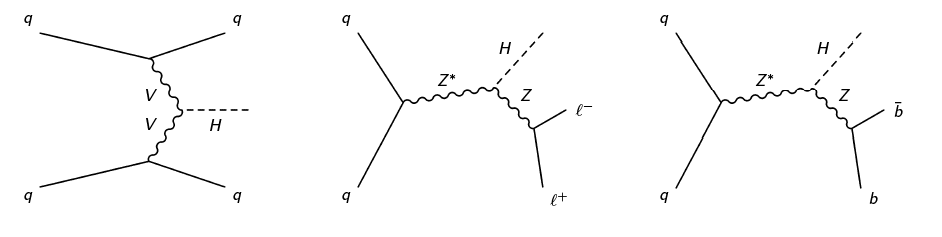
\includegraphics[width=\textwidth]{TalkPics/invcomb021213/feyndiags}
%% \begin{fmfgraph*}(100,70)
%%         \fmfleft{i1,i2}
%%         \fmfright{o1,o2,o3}
%%         \fmf{fermion}{i1,v1,o1}
%%         \fmf{fermion}{i2,v2,o3}
%%         \fmf{phantom,tension=4/5}{v1,v2}
%%         \fmffreeze
%%         \fmf{photon,label=$W,,Z$}{v1,v3}
%%         \fmf{photon,label=$W,,Z$}{v2,v3}
%%         \fmf{dashes}{v3,o2}
%%         \fmflabel{$q$}{i1}
%%         \fmflabel{$q$}{i2}
%%         \fmflabel{$q$}{o1}
%%         \fmflabel{$q$}{o3}
%%         \fmflabel{$H$}{o2}
%%       \end{fmfgraph*}
}
\date{}
\begin{document}
\begin{fmffile}{feynmandiags}

%TITLE PAGE
\section{Title}
\begin{frame}
  \titlepage

 \end{frame}

%OUTLINE                                                                                                                                                                
\begin{frame}
  \frametitle{Introduction}
  \begin{columns}
    \column{.7\textwidth}
    \begin{block}{}
      \scriptsize
  \begin{itemize}
  \item Many BSM theories predict invisible Higgs decays:
  \item[-] SUSY, Extra Dimensions, etc.
  \item Visible decays constrain invisible BF to less than 64\% at 95\% C.L.
  \item Direct searches must be performed in associated production channels
  \item There are three approved CMS Higgs to invisible results in the following channels:
  \item[-] VBF (HIG-13-013), Z($\ell\ell$)H(inv) (HIG-13-018), Z($b\bar{b}$)H(inv) (HIG-13-028)
  \item These results have been combined for a paper (HIG-13-030)
  \end{itemize}
  \end{block}
  \column{.4\textwidth}
  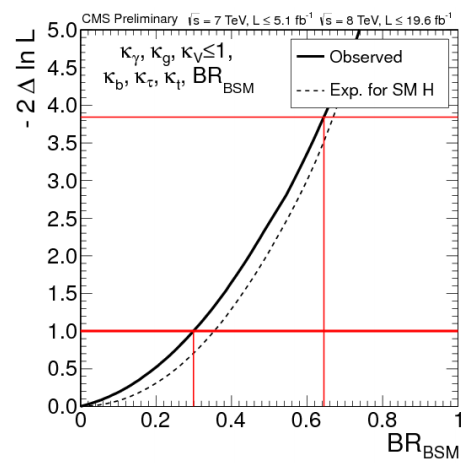
\includegraphics[width=\textwidth]{indirectbrbsm.png}
  \end{columns}
\end{frame}

 %OVERALL STRATEGY
\begin{frame}
  \frametitle{The Three Channels}
  \begin{columns}
    \column{.7\textwidth}
    \vspace{-0.7cm}
    \begin{block}{\scriptsize VBF}
      \scriptsize
    \begin{itemize}
    \item[-] Highest production cross-section
    \item[-] Difficult all hadronic final state
    \end{itemize}
    \end{block}
    \column{.3\textwidth}
    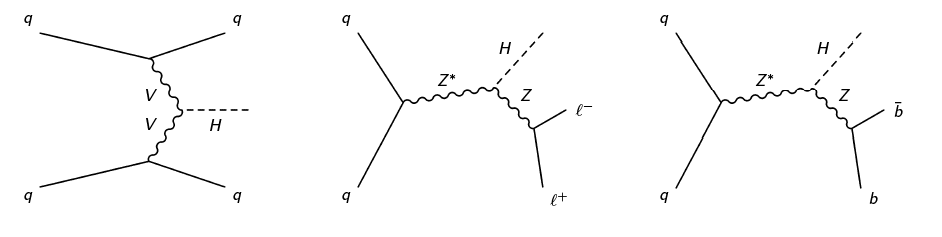
\includegraphics[clip=true,trim=0 0 460 0,height=.3\textheight]{TalkPics/invcomb021213/feyndiags}
  \end{columns}
  \begin{columns}
    \column{.7\textwidth}
    \vspace{-0.7cm}
    \begin{block}{\scriptsize Z($\ell\ell$)H(inv)}
      \scriptsize
    \begin{itemize}
    \item[-] Production cross-section lower than VBF
    \item[-] Clean all leptonic final state
    \end{itemize}
    \end{block}
    \column{.3\textwidth}
    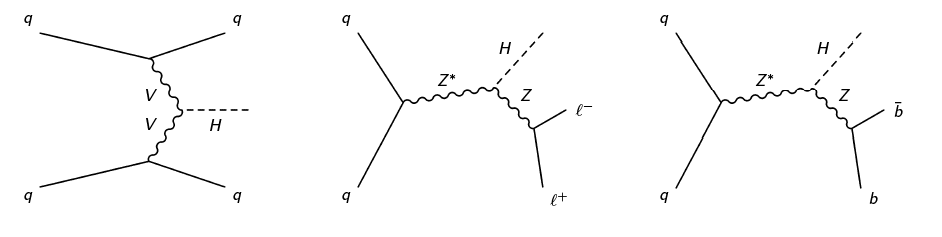
\includegraphics[clip=true,trim=235 0 220 0,height=.3\textheight]{TalkPics/invcomb021213/feyndiags}
  \end{columns}
  \begin{columns}
    \column{.7\textwidth}
    \vspace{-0.7cm}
    \begin{block}{\scriptsize Z($b\bar{b}$)H(inv)}
      \scriptsize
    \begin{itemize}
    \item[-] Also much lower production cross-section than VBF
    \item[-] Same final state as Z(inv)H($b\bar{b}$)
    \end{itemize}
    \end{block}
    \column{.3\textwidth}
    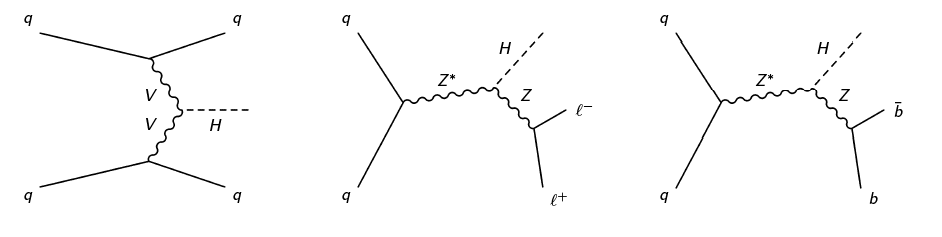
\includegraphics[clip=true,trim=470 0 0 0,height=.3\textheight]{TalkPics/invcomb021213/feyndiags}
  \end{columns}
\end{frame}

 \begin{frame}%
   \frametitle{VBF Measurement Strategy}
   \begin{columns}
     \column{.5\textwidth}
     \vspace{-.2cm}
     \scriptsize
     \begin{block}{\scriptsize General Strategy}
       \begin{itemize}
       \item Clean data from pileup and mismeasured MET
       \item Use hard cuts to restrict backgrounds
       \item Remaining background estimation must be data driven as hard cuts make MC unreliable
       \end{itemize}
     \end{block}

     \vspace{-.15cm}

    \begin{block}{\scriptsize Main backgrounds:}
      \scriptsize
      \begin{itemize}
      \item $W$ + jets where lepton is missed
      \item $Z\rightarrow\nu\nu$ + jets
      \item QCD
      \end{itemize}
    \end{block}

     \column{.5\textwidth}
     \centering
     \begin{block}{\scriptsize Select VBF Topology}
       \scriptsize
       \begin{itemize}
       \item 2 jets with a large $\eta$ separation
       \item Nothing in the gap between the jets
       \item Need dedicated VBF trigger
       \end{itemize}
     \end{block}

     \vspace{-0.3cm}

     \begin{block}{\scriptsize Cuts}
       \scriptsize
       \begin{itemize}
       \item Require 2 jets in all regions:
       \item[-] Both jets must pass loose PUJetID
       \item[-] $p_{T} > 50 GeV$,  $|\eta| < 4.7$
       \item[-] $|\Delta\eta|>4.2$ , $\eta_{j_{1}}*\eta_{j{_2}}<0$
       \item[-] $m_{jj} > 1100 GeV$
       \item Central Jet Veto (CJV)
       \item[-] Veto events with jets with $p_{T}>30$GeV between the tag jets unless stated otherwise
      \end{itemize}
     \end{block}

     
  \end{columns}
\end{frame}

%SIGNAL EVENT SELECTION
\begin{frame} 
  \frametitle{VBF Signal Event Selection}
  \vspace{-0.2cm}
  \begin{block}{\scriptsize Signal Region Selection:}
    \scriptsize
    \begin{itemize}
    \item PFMET $> 130GeV$, $\Delta\phi_{jj}<1.0$ to reduce QCD
    \item $e/\mu$ veto to reduce $W/Z$+jets
    \end{itemize}
  \end{block}
  \vspace{-0.15cm}
  \begin{columns}
    \column{.5\textwidth}
    \column{.5\textwidth}
    \scriptsize Data MC difference is QCD
  \end{columns}
  \begin{columns}
    \column{.5\textwidth}
    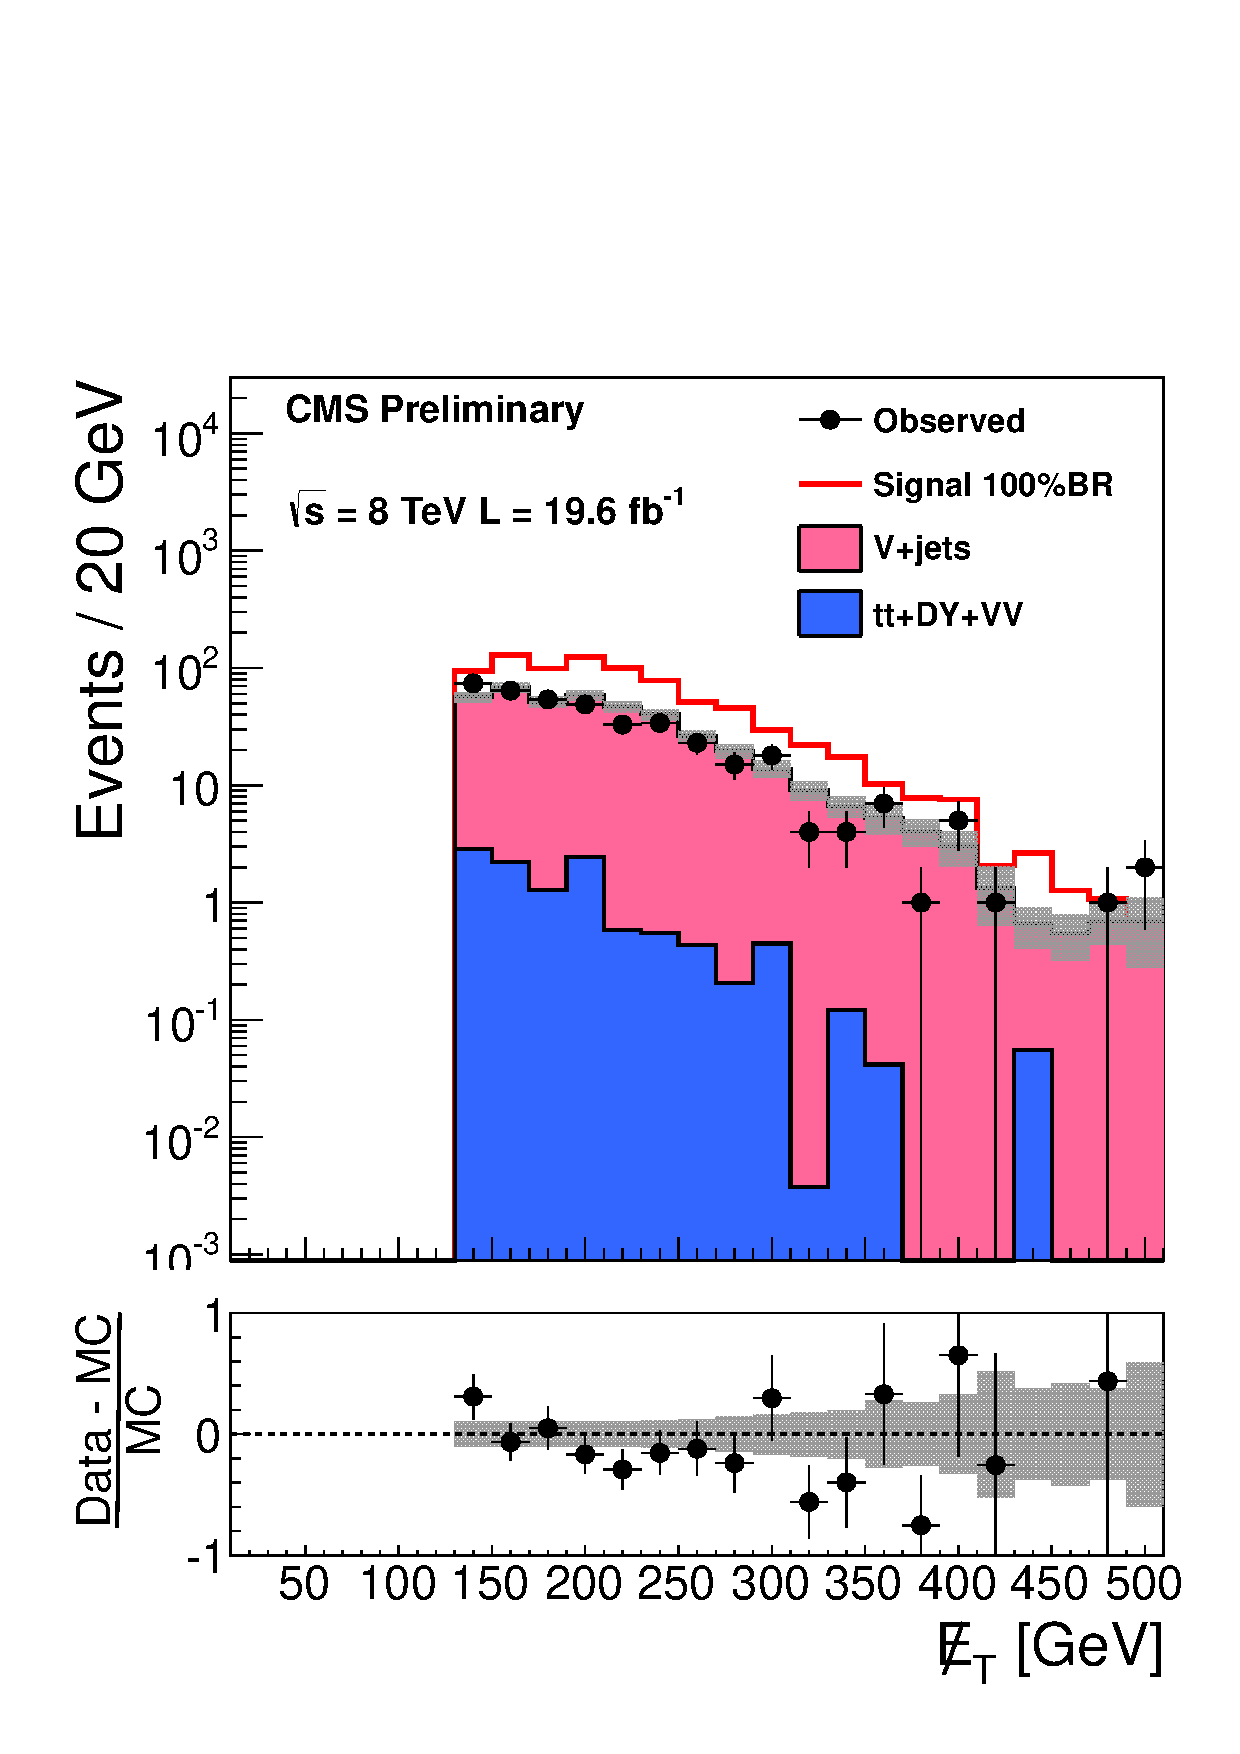
\includegraphics[width=\textwidth,height=.5\textheight]{TalkPics/iccms091013/hMETNM1.pdf}
    \column{.5\textwidth}
    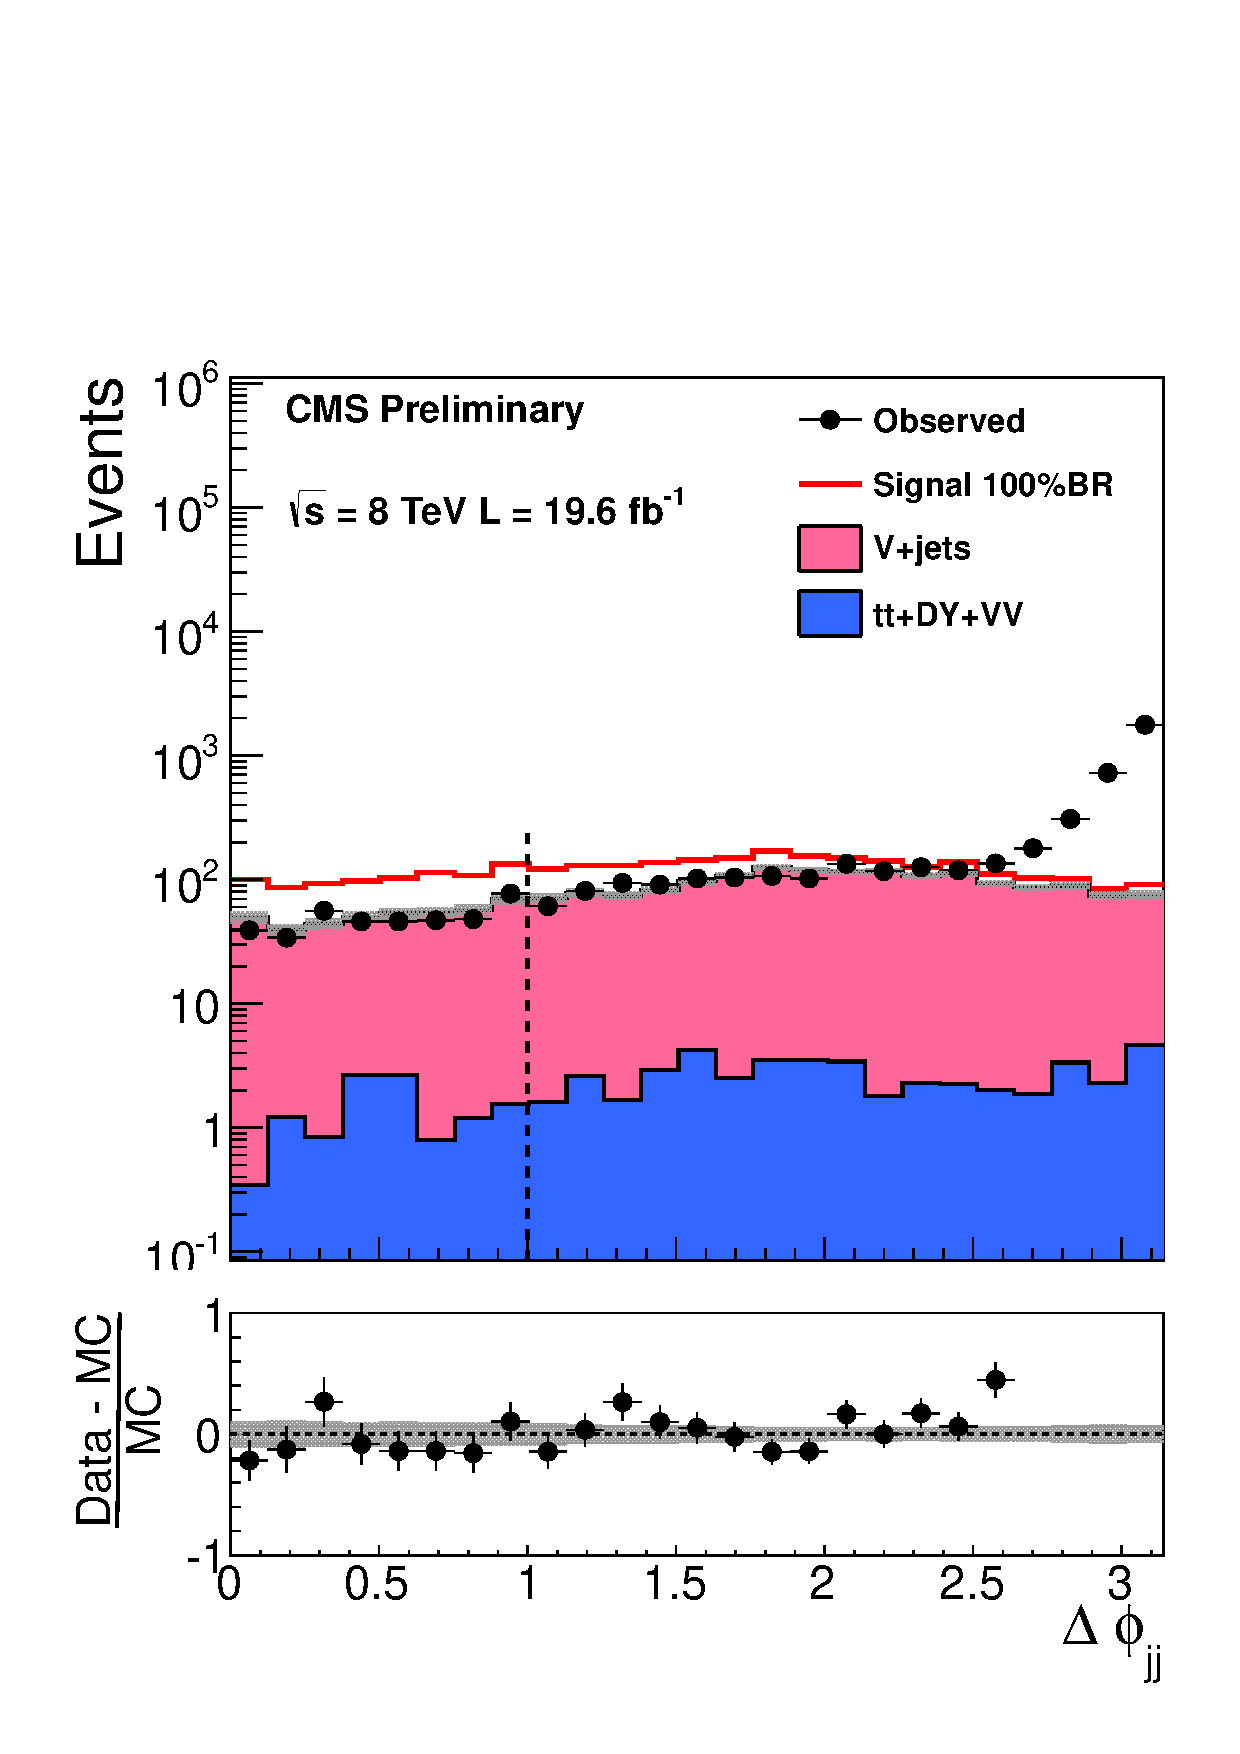
\includegraphics[width=\textwidth,height=.5\textheight]{TalkPics/iccms091013/hDPhiJJNM1.pdf}
  \end{columns}
\tiny
\vspace{-0.1cm}
\end{frame}



\begin{frame}%!!PUT RESULTS IN
  \frametitle{VBF W/Z + jets Background Estimation}
  \begin{columns}
    \column{.6\textwidth}
    \vspace{-0.3cm}
    \begin{block}{\scriptsize Data Driven Estimation Method:}
      \scriptsize
      \begin{itemize}
      \item Pick $W/Z$ dominated control region in same trigger sample with same VBF selection
      \item[-] For muons recalculate MET after removing leptons from $W$ \& $Z$ to mimic $W$ with missed muon/$Z\rightarrow\nu\nu$
      \item Check data/MC shape agreement in control regions
      \item Assume MC signal/control ratio is the same as that in data
      \end{itemize}
    \end{block}

    \vspace{-0.3cm}

    \begin{block}{\scriptsize Results}
      \scriptsize
      \begin{itemize}
        \item $W\rightarrow e\nu$: 62.7 $\pm$ 8.7 (stat.) $\pm$ 8.6 (syst.)
        \item $W\rightarrow\mu\nu$: 66.8 $\pm$ 5.2 (stat.) $\pm$ 7.0 (syst.)
        \item $W\rightarrow\tau\nu$: 53 $\pm$ 18 (stat.) $\pm$ 14 (syst.)
        \item $Z\rightarrow\nu\nu$: 103 $\pm$ 30 (stat.) $\pm$ 14 (syst.)
      \end{itemize}
    \end{block}
    \column{.4\textwidth}
    \begin{block}{\scriptsize $W \rightarrow \mu/ e$ Control Region:}
      \scriptsize
      \begin{itemize}
      \item 1 tight muon/electron:
      \item MET $>130 GeV$
      \end{itemize}
    \end{block}

    \vspace{-0.3cm}

    \begin{block}{\scriptsize $W\rightarrow \tau$ Control Region:}
      \scriptsize
      \begin{itemize}
      \item Remove CJV
      \item Require 1 $\tau_{hadronic}$ candidate
      \end{itemize}
    \end{block}

    \vspace{-0.3cm}

    \begin{block}{\scriptsize $Z\rightarrow\nu\nu$ Control Region:}
      \scriptsize
      \begin{itemize}
      \item Require 2 tight muons with $60<M_{\mu\mu}<120$ GeV
      \item MET without $Z$ candidate $> 130 GeV$
      \item Correct for different cross-section for the two processes
      \end{itemize}
    \end{block}
    
  \end{columns}
\end{frame}

%QCD
\begin{frame}%!!UPDATE
  \frametitle{VBF QCD Estimation}
  \begin{columns}
    \column{.5\textwidth}
    \begin{block}{\scriptsize QCD Background Strategy}
      \scriptsize
      \begin{itemize}
      \item V. low MC statistics
      \item[1)] Reduce background with cuts
      \item[2)] Estimate using data driven ABCD method in MET and CJV
      \item[3)] Cross-check using ABCD method in MET and $\Delta\phi_{jj}$
            \end{itemize}
    \end{block}
    \begin{block}{\scriptsize QCD ABCD method:}
      \scriptsize
      \begin{itemize}
      \item Choose 4 regions:
      \end{itemize}
      \begin{tabular}{|l|c|c|}
        \hline
        & Fail MET & Pass MET \\
        \hline
        Fail CJV & A & B \\
        \hline
        Pass CJV & C & D (signal) \\
        \hline
      \end{tabular}
      \begin{itemize}
      \item $N_{D}=N_{B}N_{C}/N_{A}$
      \end{itemize}
    \end{block}
    \column{.5\textwidth}
    \begin{block}{}
      \scriptsize
      \begin{itemize}
      \item $N_{QCD}=$32.5 $\pm$ 5.6 (stat.) $\pm$ 13.0 (syst.)
      \end{itemize}
    \end{block}

    \vspace{.5cm}

    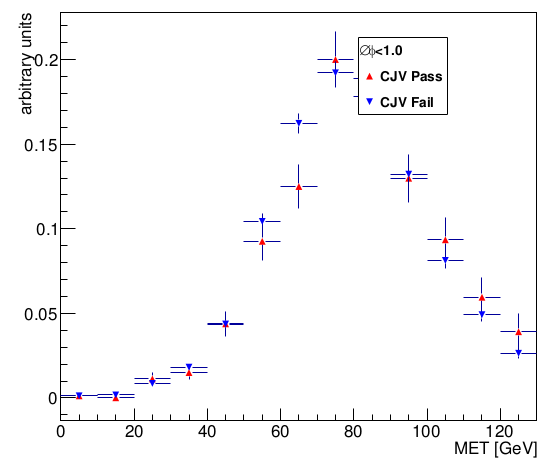
\includegraphics[width=\textwidth,height=.6\textheight]{TalkPics/iccms091013/qcdmet.png}
  \end{columns}
\end{frame}



\begin{frame}
  \frametitle{Combination Method}
  \begin{block}{}
    \scriptsize
  \begin{itemize}
  \item Datacards for the three channels were combined using the standard Higgs combination tool
  \item The following uncertainties were considered correlated between channels in decreasing order of importance:
  \end{itemize}
  \end{block}

  \begin{block}{}
      \scriptsize
      \center
    \begin{tabular}{|l|c|}
      \hline
      Nuisance & Analyses which it affects \\
      \hline
      Jet energy scale & VBF, Z($\ell\ell$)H(inv) \\
      PDF uncertainties & VBF, Z($b\bar{b}$), Z($\ell\ell$)H(inv) \\
      QCD scale & VBF, Z($b\bar{b}$), Z($\ell\ell$)H(inv) \\
      Luminosity & VBF, Z($b\bar{b}$)H(inv), Z($\ell\ell$)H(inv) \\
      Jet energy resolution & VBF, Z($\ell\ell$)H(inv) \\
      Unclustered energy scale & VBF, Z($b\bar{b}$)H(inv), Z($\ell\ell$)H(inv) \\
      Muon identification efficiency & VBF, Z($\ell\ell$)H(inv) \\
      Electron identification efficiency & VBF, Z($\ell\ell$)H(inv) \\
      \hline
    \end{tabular}
    \end{block}
\end{frame}

\begin{frame}
  \frametitle{Separate results: Cross-Section limits}
  \centering
  \begin{columns}
    \column{.5\textwidth}
    \begin{itemize}
    \item VBF
    \end{itemize}
    \column{.5\textwidth}
    \begin{itemize}
    \item ZH
    \end{itemize}
  \end{columns}
  \begin{columns}
    \column{.5\textwidth}
    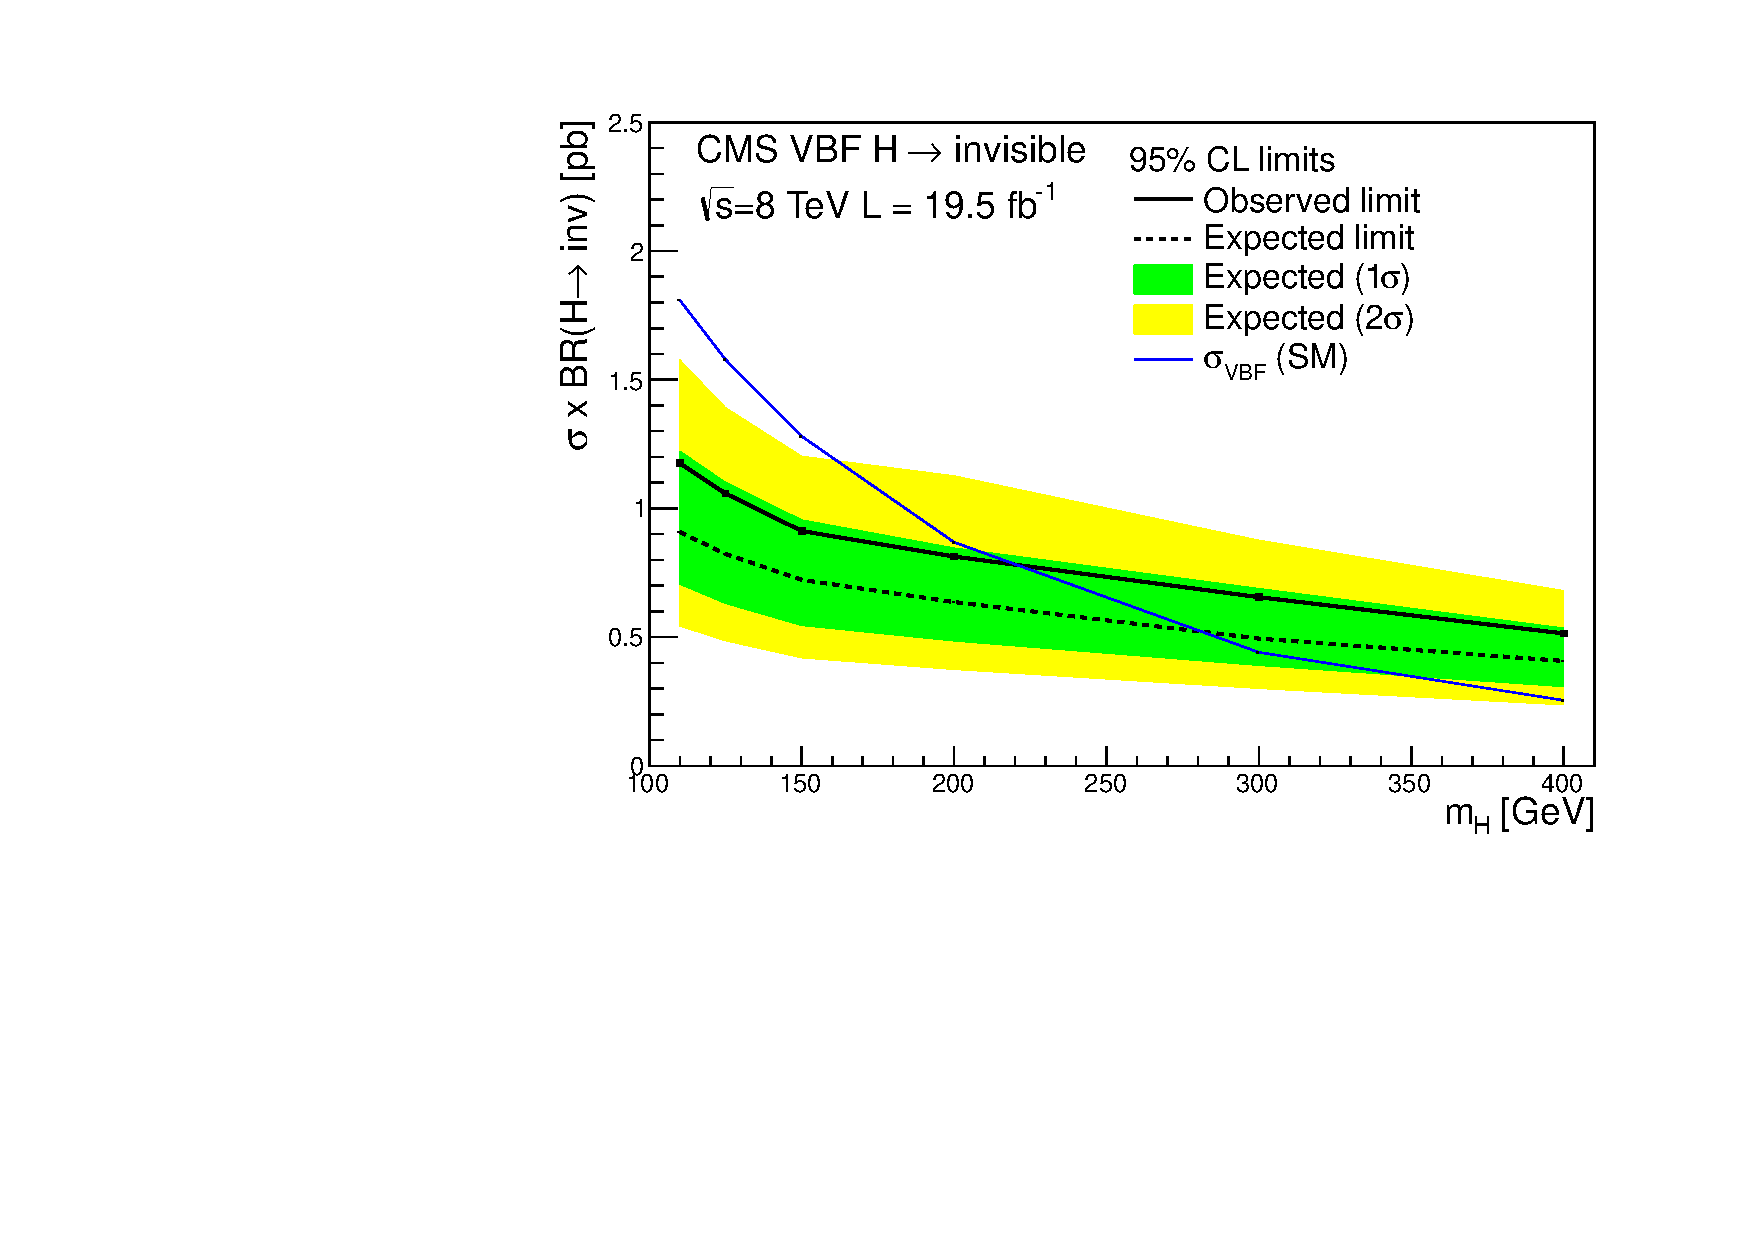
\includegraphics[width=\textwidth]{TalkPics/invcomb021213/vbfxslimit.pdf}
    \column{.5\textwidth}
    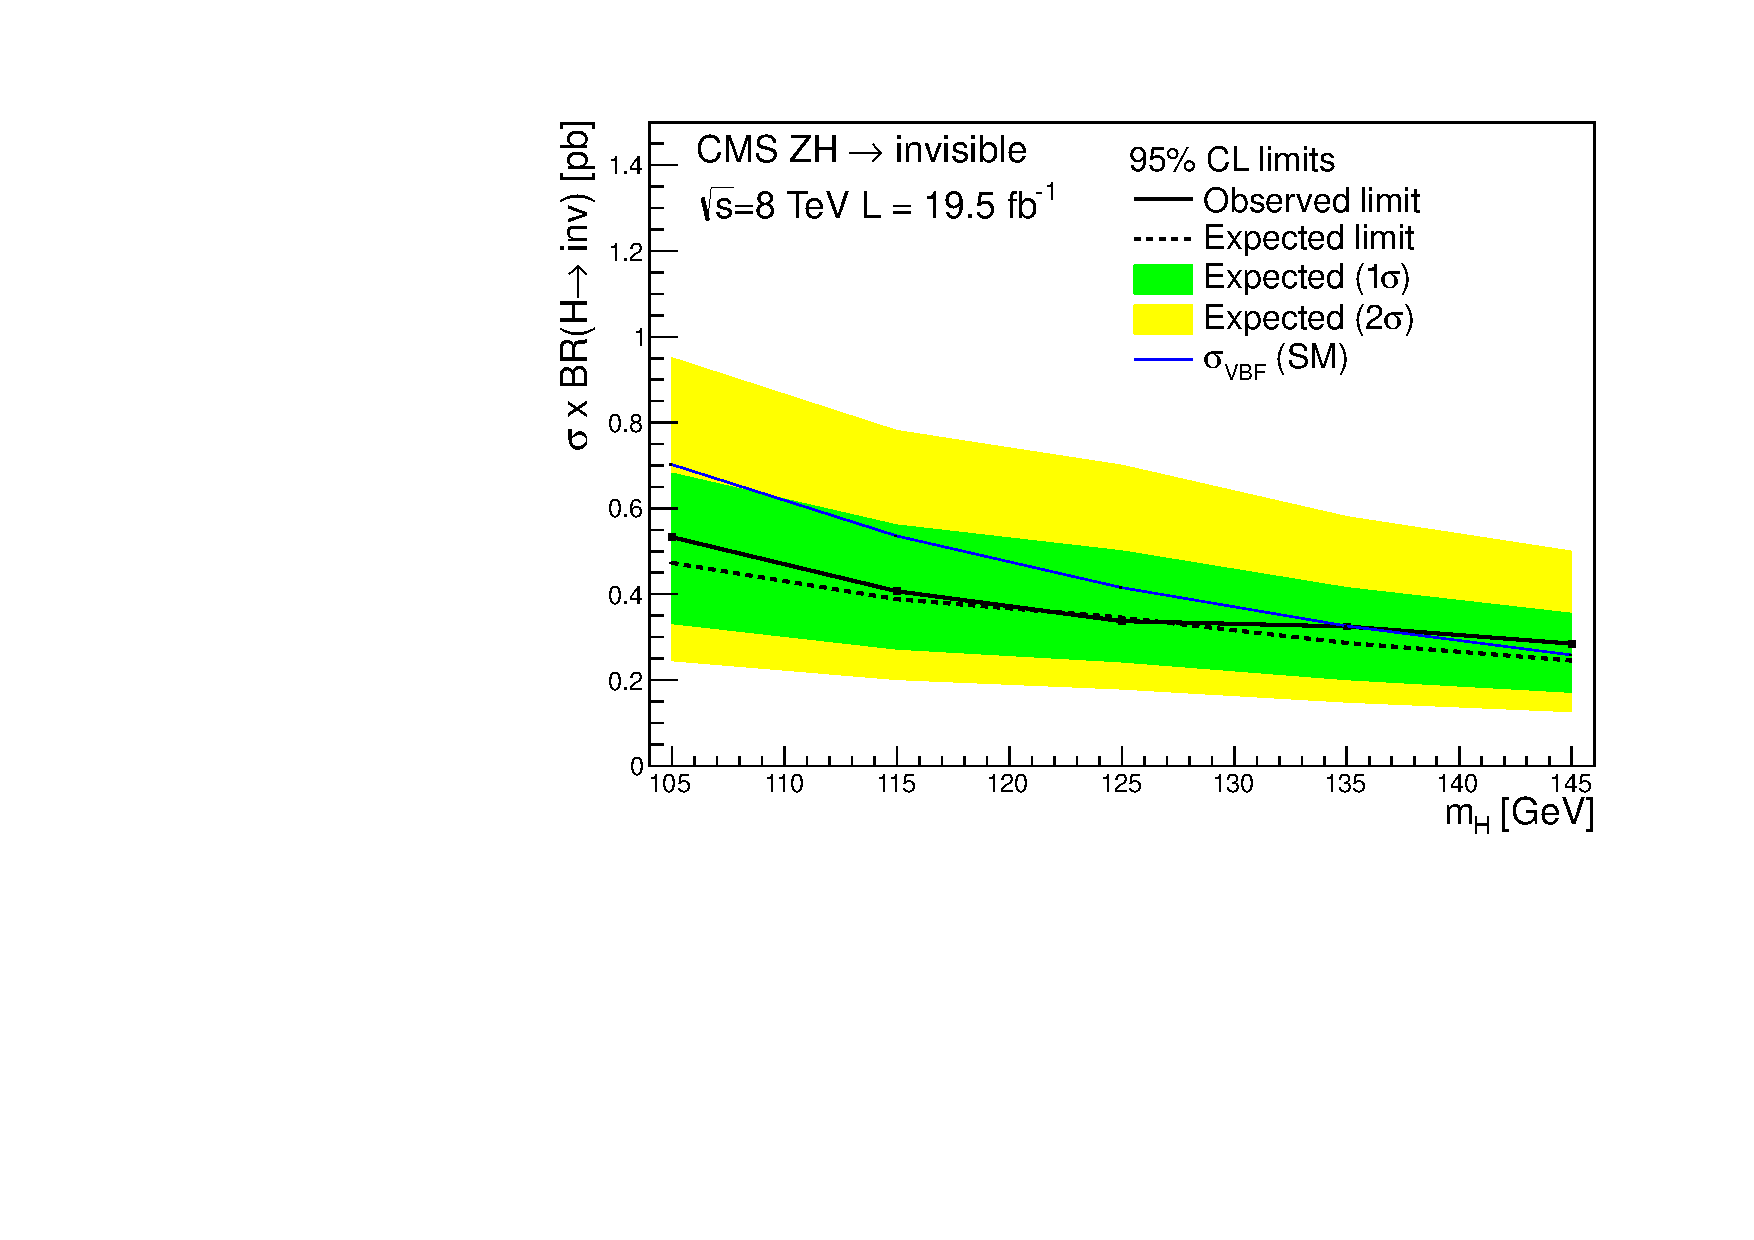
\includegraphics[width=\textwidth]{TalkPics/invcomb021213/zhxslimit.pdf}
  \end{columns}
  \begin{columns}
    \column{.5\textwidth}
    \begin{block}{}
      \scriptsize
    \begin{itemize}
    \item Observed (expected) limit of 67\% (52\%) at 95\% C.L. on $BR_{inv}$ for a 125 GeV Higgs
    \end{itemize}
    \end{block}
    \column{.5\textwidth}
    \begin{block}{}
      \scriptsize
    \begin{itemize}
    \item Observed (expected) limit of 81\% (83\%) at 95\% C.L. on $BR_{inv}$ for a 125 GeV Higgs
    \end{itemize}
    \end{block}
  \end{columns}
\end{frame}

\begin{frame}
  \frametitle{Separate results: Direct}
  \centering
  \begin{columns}
    \column{.5\textwidth}
    \begin{itemize}
    \item VBF
    \end{itemize}
    \column{.5\textwidth}
    \begin{itemize}
    \item ZH
    \end{itemize}
  \end{columns}
  \begin{columns}
    \column{.5\textwidth}
    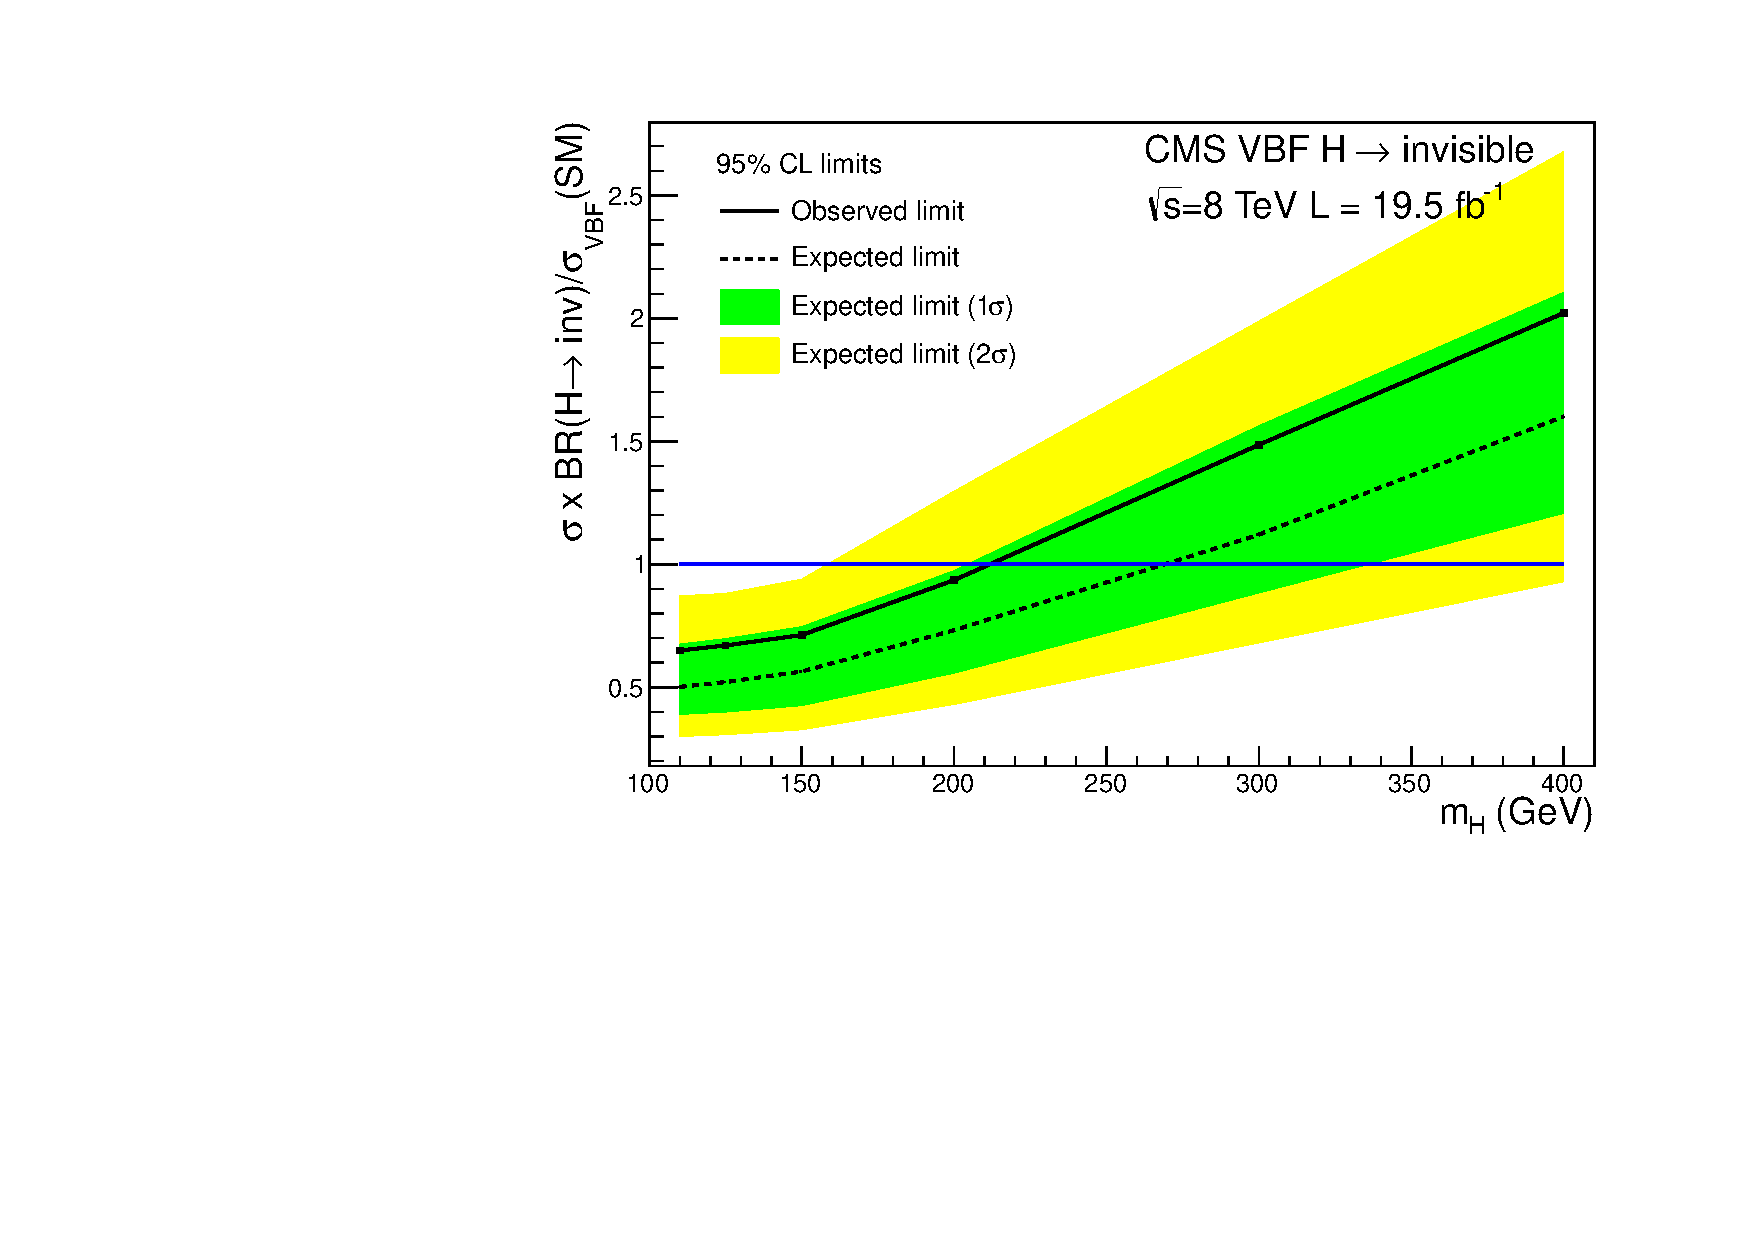
\includegraphics[width=\textwidth]{TalkPics/invcomb021213/vbflimit.pdf}
    \column{.5\textwidth}
    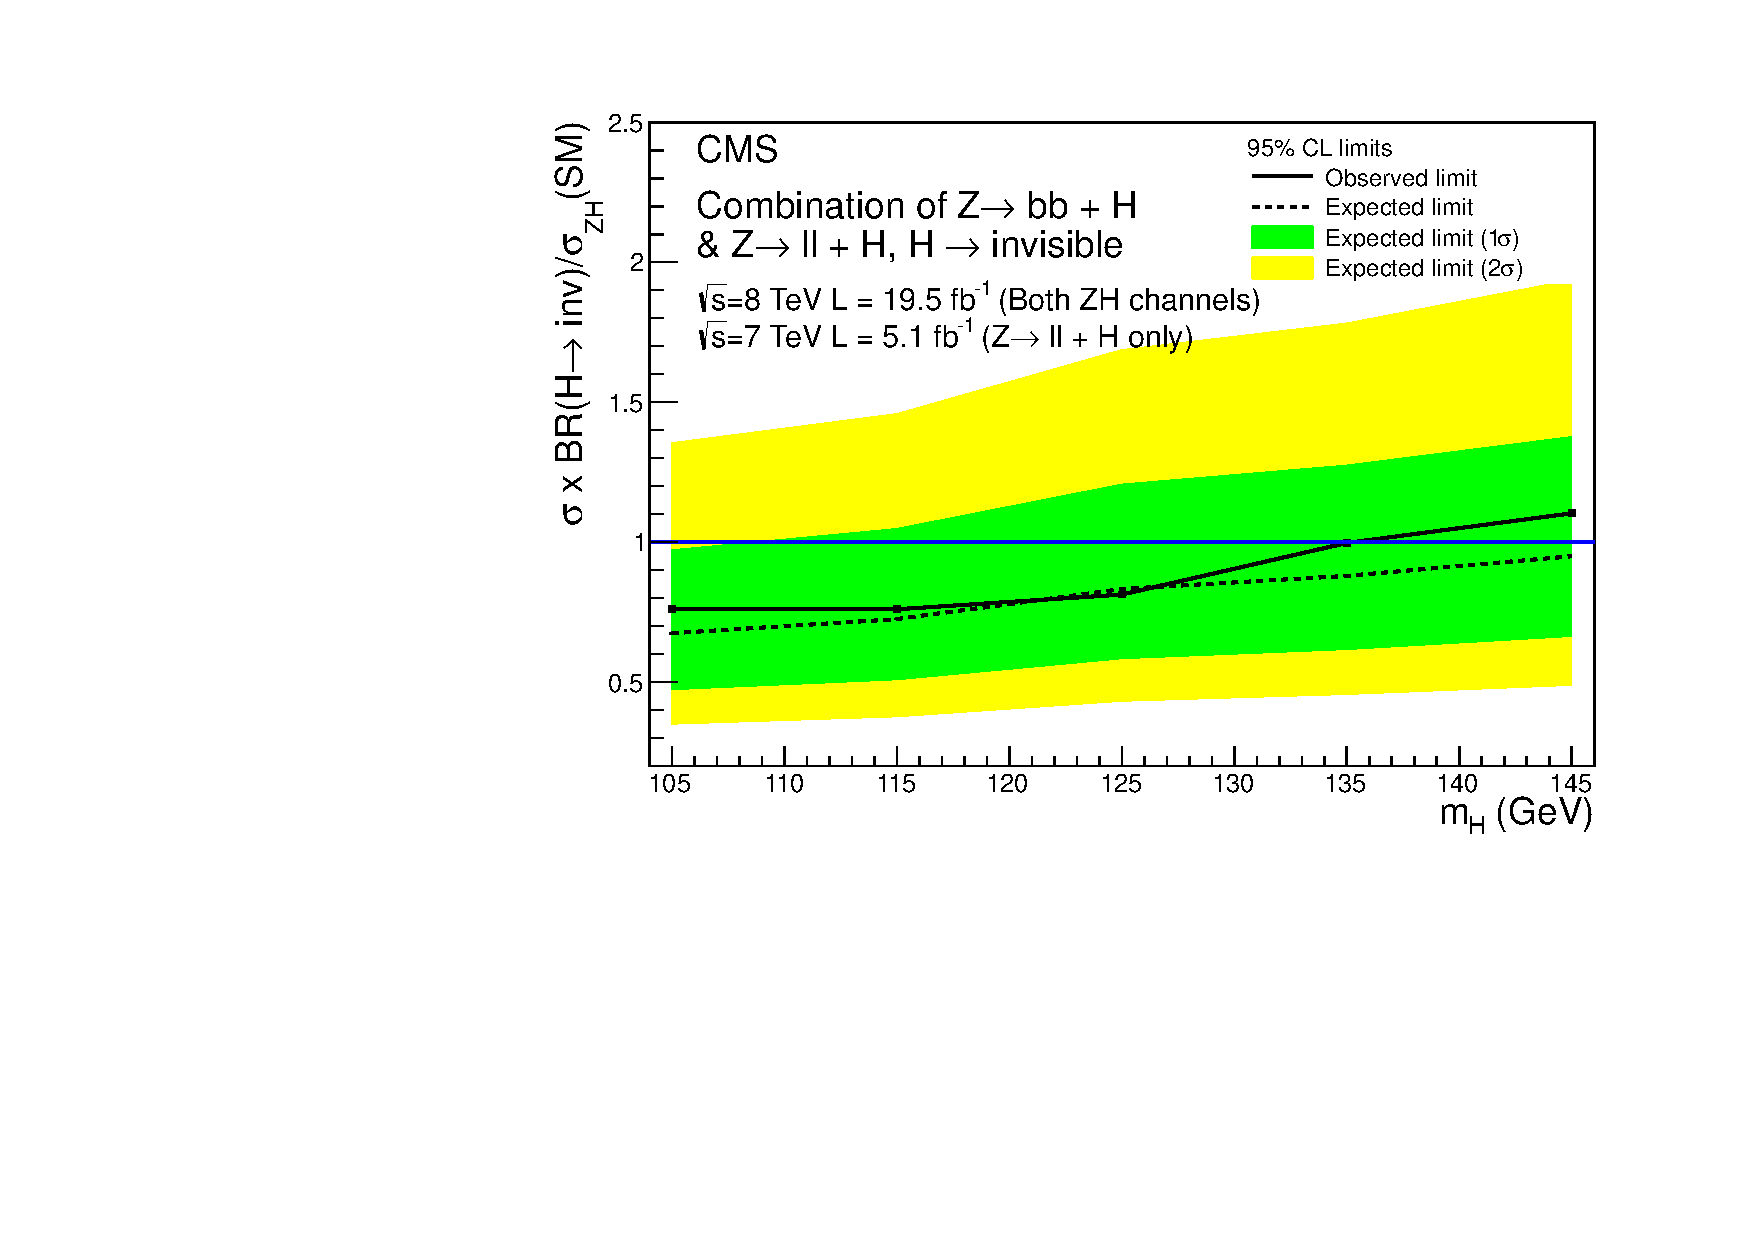
\includegraphics[width=\textwidth]{TalkPics/invcomb021213/zhlimit.pdf}
  \end{columns}
  \begin{columns}
    \column{.5\textwidth}
    \begin{block}{}
      \scriptsize
    \begin{itemize}
    \item Observed (expected) limit of 67\% (52\%) at 95\% C.L. on $BR_{inv}$ for a 125 GeV Higgs
    \end{itemize}
    \end{block}
    \column{.5\textwidth}
    \begin{block}{}
      \scriptsize
    \begin{itemize}
    \item Observed (expected) limit of 81\% (83\%) at 95\% C.L. on $BR_{inv}$ for a 125 GeV Higgs
    \end{itemize}
    \end{block}
  \end{columns}
\end{frame}

\begin{frame}
  \frametitle{Combined Results}
  \centering
  %\vspace{-.2cm}
  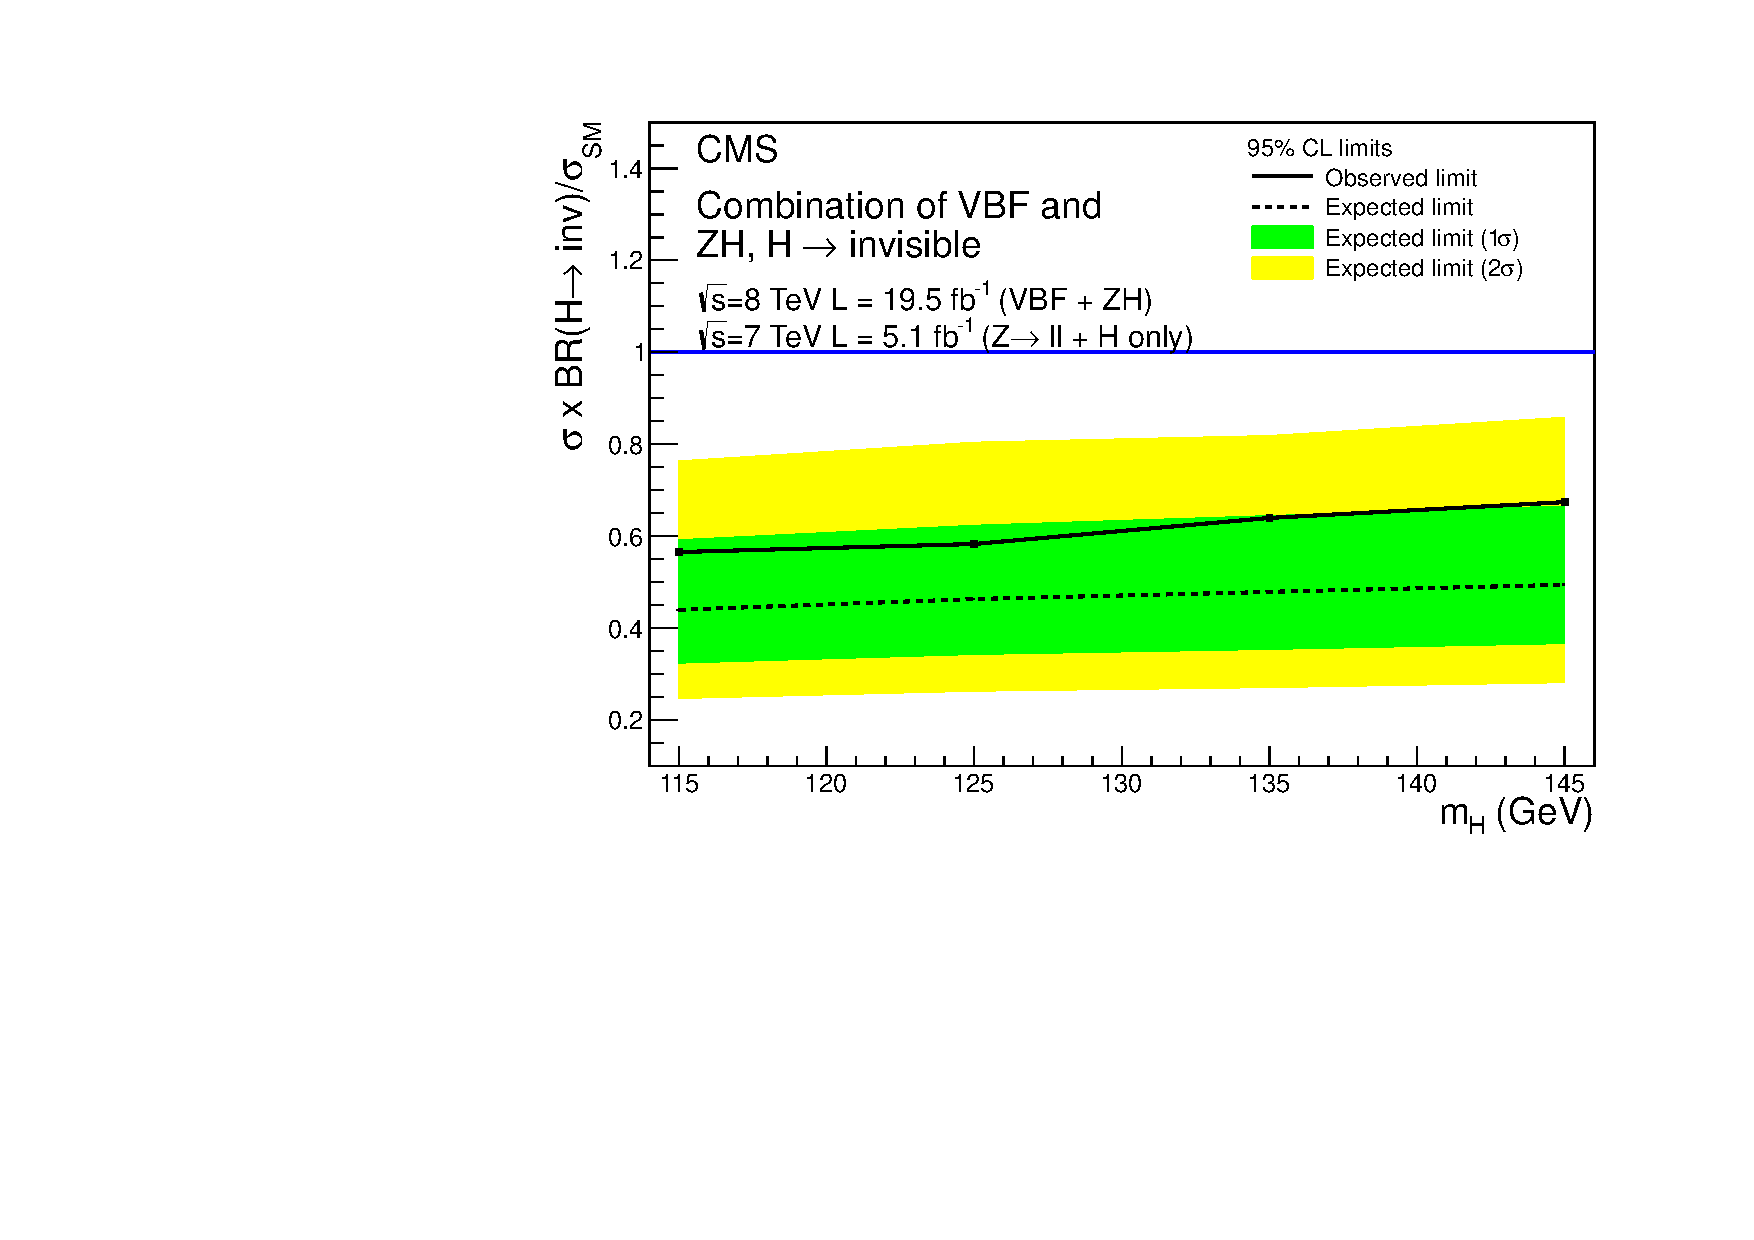
\includegraphics[clip=true,trim=0 5 0 20, width=.8\textwidth]{TalkPics/invcomb021213/combinedlimit.pdf}
  \vspace{-.3cm}
  \begin{block}{}
    \scriptsize
  \begin{itemize}
  \item Observed (expected) limit at 125 GeV is 58(46)\%
  \item[-] Combination between direct and indirect methods is being investigated
  \end{itemize}
  \end{block}
\end{frame}

\begin{frame}
  \frametitle{Other Interpretations}
  \centering
  \vspace{-.3cm}
  \begin{columns}
    \column{.5\textwidth}
  \begin{block}{}
    \scriptsize
  \begin{itemize}
  \item Z($\ell\ell$)H(inv) and VBF both have datacards up to 300 GeV
  \item The method above was used to combine these two channels between 115 and 300 GeV
  \end{itemize}
  \end{block}
  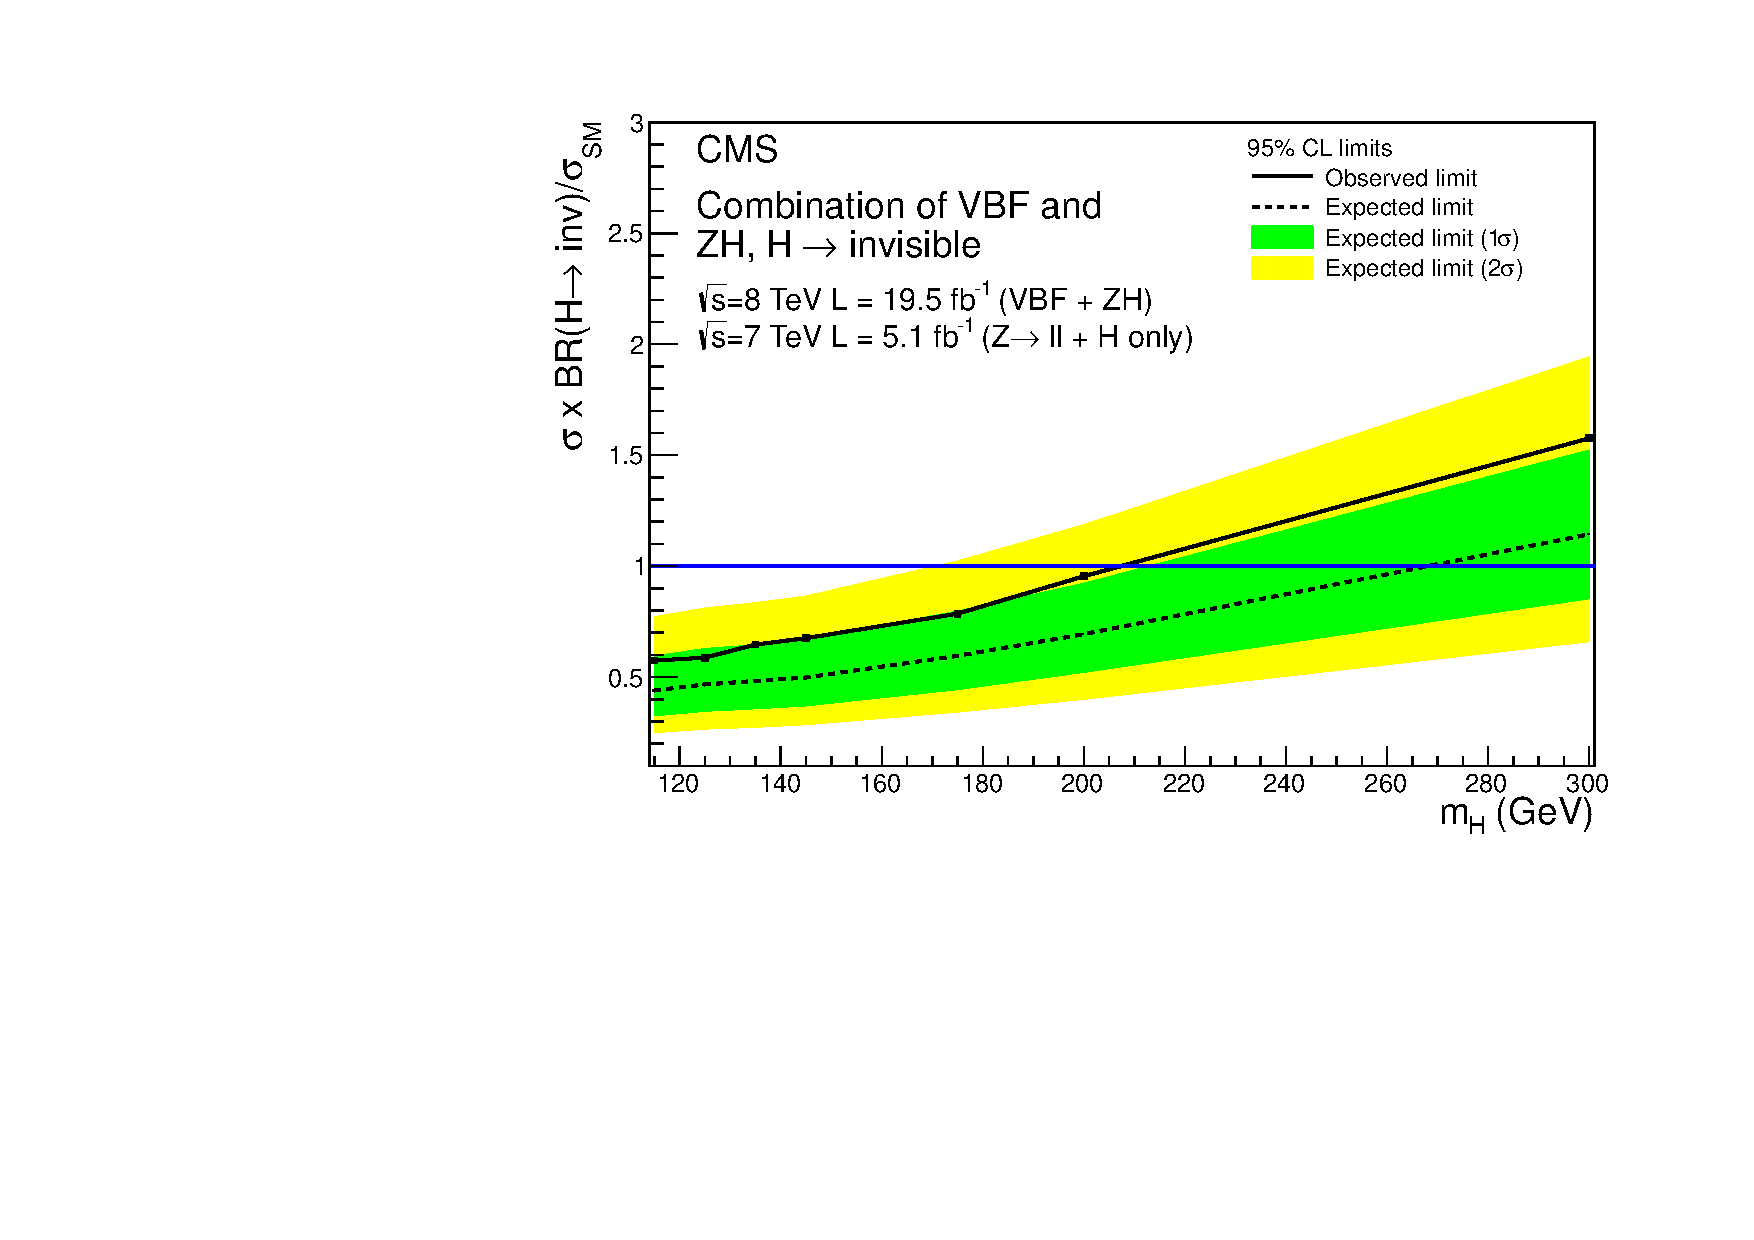
\includegraphics[clip=true,trim=0 5 0 20, width=1.1\textwidth]{TalkPics/invcomb021213/highmasslimit.pdf}
  \column{.5\textwidth}
  \vspace{0.2cm}
  \begin{block}{}
      \scriptsize
      \begin{itemize}
      \item Limits can also be interpreted as constraints on dark matter models (arXiv:1205.3169)
      \item Competitive with dedicated experiments at very low mass
      \end{itemize}
    \end{block}

    %\vspace{.6cm}

    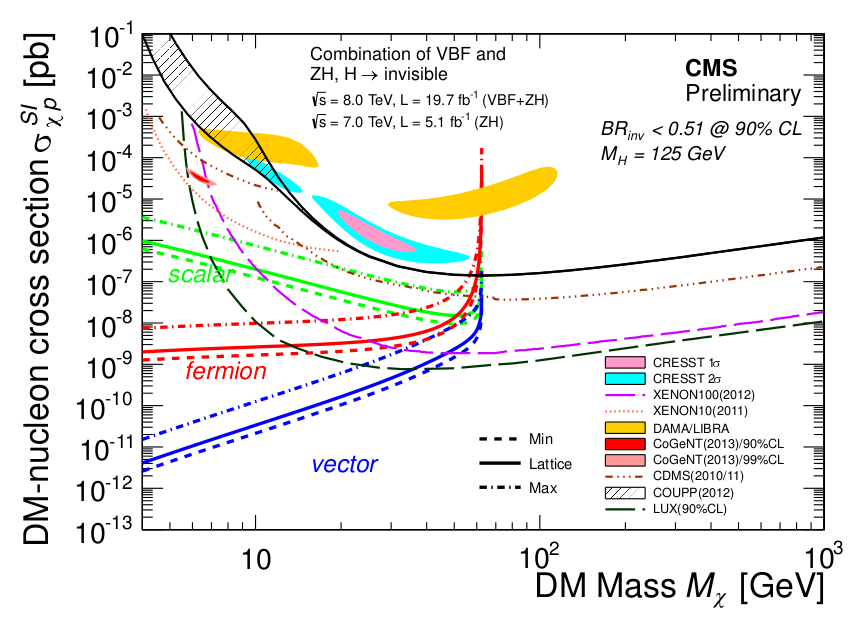
\includegraphics[width=\textwidth]{TalkPics/cmsuk080114/dmlimit1.png}
  \end{columns}
 \end{frame}

\begin{frame}
  \frametitle{Conclusions}
  \label{lastframe}
  \begin{columns}
    \column{.5\textwidth}
    \vspace{-0.3cm}
    \begin{block}{}
      \scriptsize
      \begin{itemize}
      \item All three H$\rightarrow$invisible channels have been combined using the standard Higgs combination tool
      \item The result is compatible with the SM
      \item The combined result gives the strongest limit on the invisible branching fraction of the 125 GeV Higgs
      \end{itemize}
    \end{block}
    
    \vspace{-0.3cm}
    \begin{block}{\footnotesize Plans}
      \scriptsize
      \begin{itemize}
      \item A paper for the prompt data has just finished CWR
      \item An improved analysis is planned using the parked data
      \end{itemize}
    \end{block}
    

    \column{.5\textwidth}
    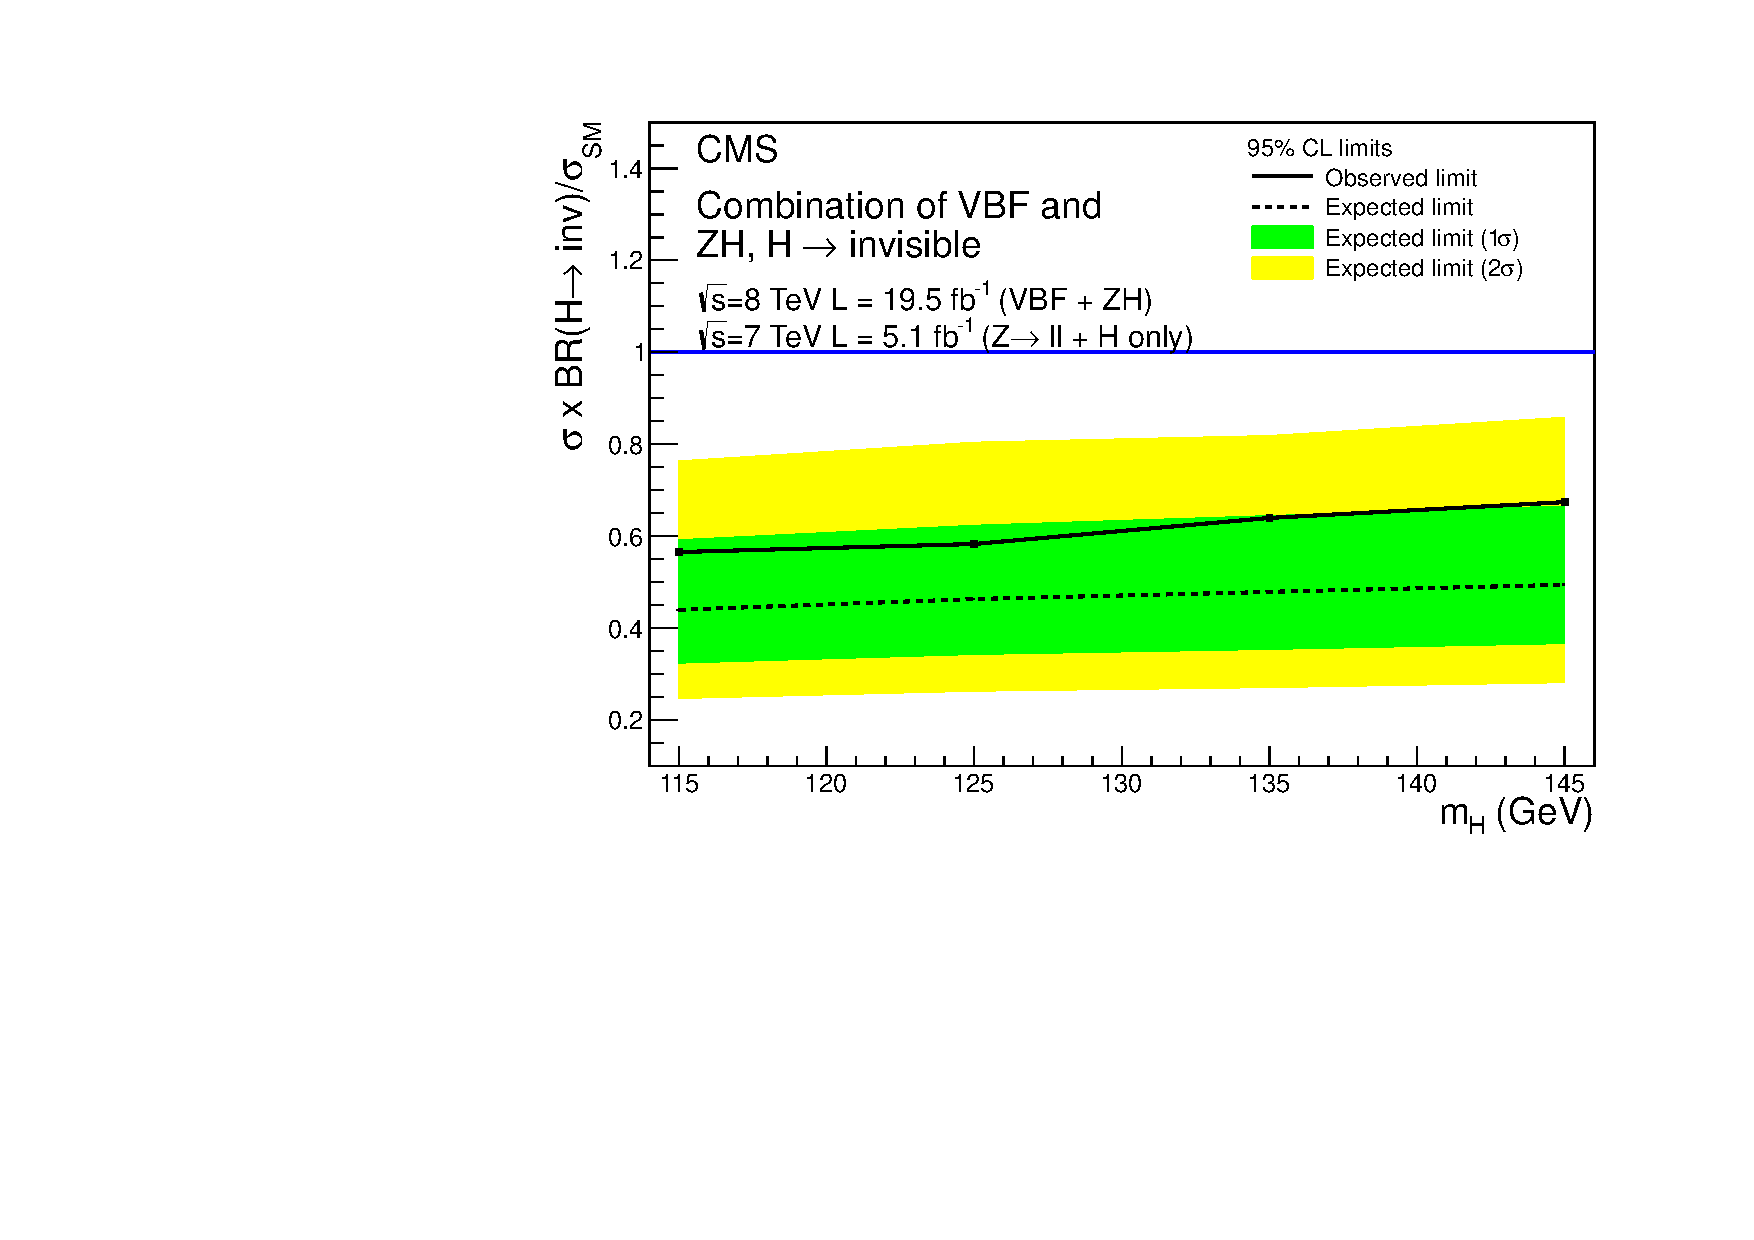
\includegraphics[clip=true,trim=0 5 0 20, width=1.2\textwidth]{TalkPics/invcomb021213/combinedlimit.pdf}
  \end{columns}
\end{frame}

%!!UPDATE

\begin{frame}%!! UPDATE ALL BACKUP
  \frametitle{BACKUP}
\end{frame}

\begin{frame}%!!UPDATE MAYBE TRIM
  \frametitle{Datacards}
  \begin{itemize}
    \item All three channels have signal MC at different mass points
  \end{itemize}
  \begin{center}
  \begin{tabular}{|l|c|}
    \hline
    Channel & Mass Points/GeV \\
    \hline
    Z($\ell\ell$)H(inv) & 105, 115, 125, 135, 145, 175, 200 \& 300 \\
    Z($b\bar{b}$)H(inv) & 105, 115, 125, 135, 145 \& 150 \\
    VBF & 110, 125, 150, 200, 300 \& 400 \\
    \hline
  \end{tabular}
  \end{center}
  \begin{itemize}
  \item New VBF datacards were produced for 115,135 and 145 GeV
  \item[-] Nuisances are linearly interpolated between mass points.
  \item[-] Signal yields are interpolated using the method described below.
  \end{itemize}
  \begin{itemize}
  \item[-] Combination between direct and indirect methods is being investigated e.g. \href{https://indico.cern.ch/getFile.py/access?contribId=3&sessionId=9&resId=1&materialId=slides&confId=267834}{talk by M. Zanetti}
  \end{itemize}
\end{frame}

\begin{frame}%!!MAYBE MOVE TO BACKUP
  \frametitle{Signal Yield interpolation}
  \begin{columns}
    \column{.5\textwidth}
    \begin{itemize}
    \item $N_{Signal}=eff. \times acc. \times \mathcal L\sigma$
    \item Luminosity is constant
    \item Yield over cross-section is thus proportional to efficiency times acceptance
    \item[-] Cross-sections from LHC-HXSWG were used
    \end{itemize}
    \column{.5\textwidth}
    \centering
    \hspace{-.5cm}
    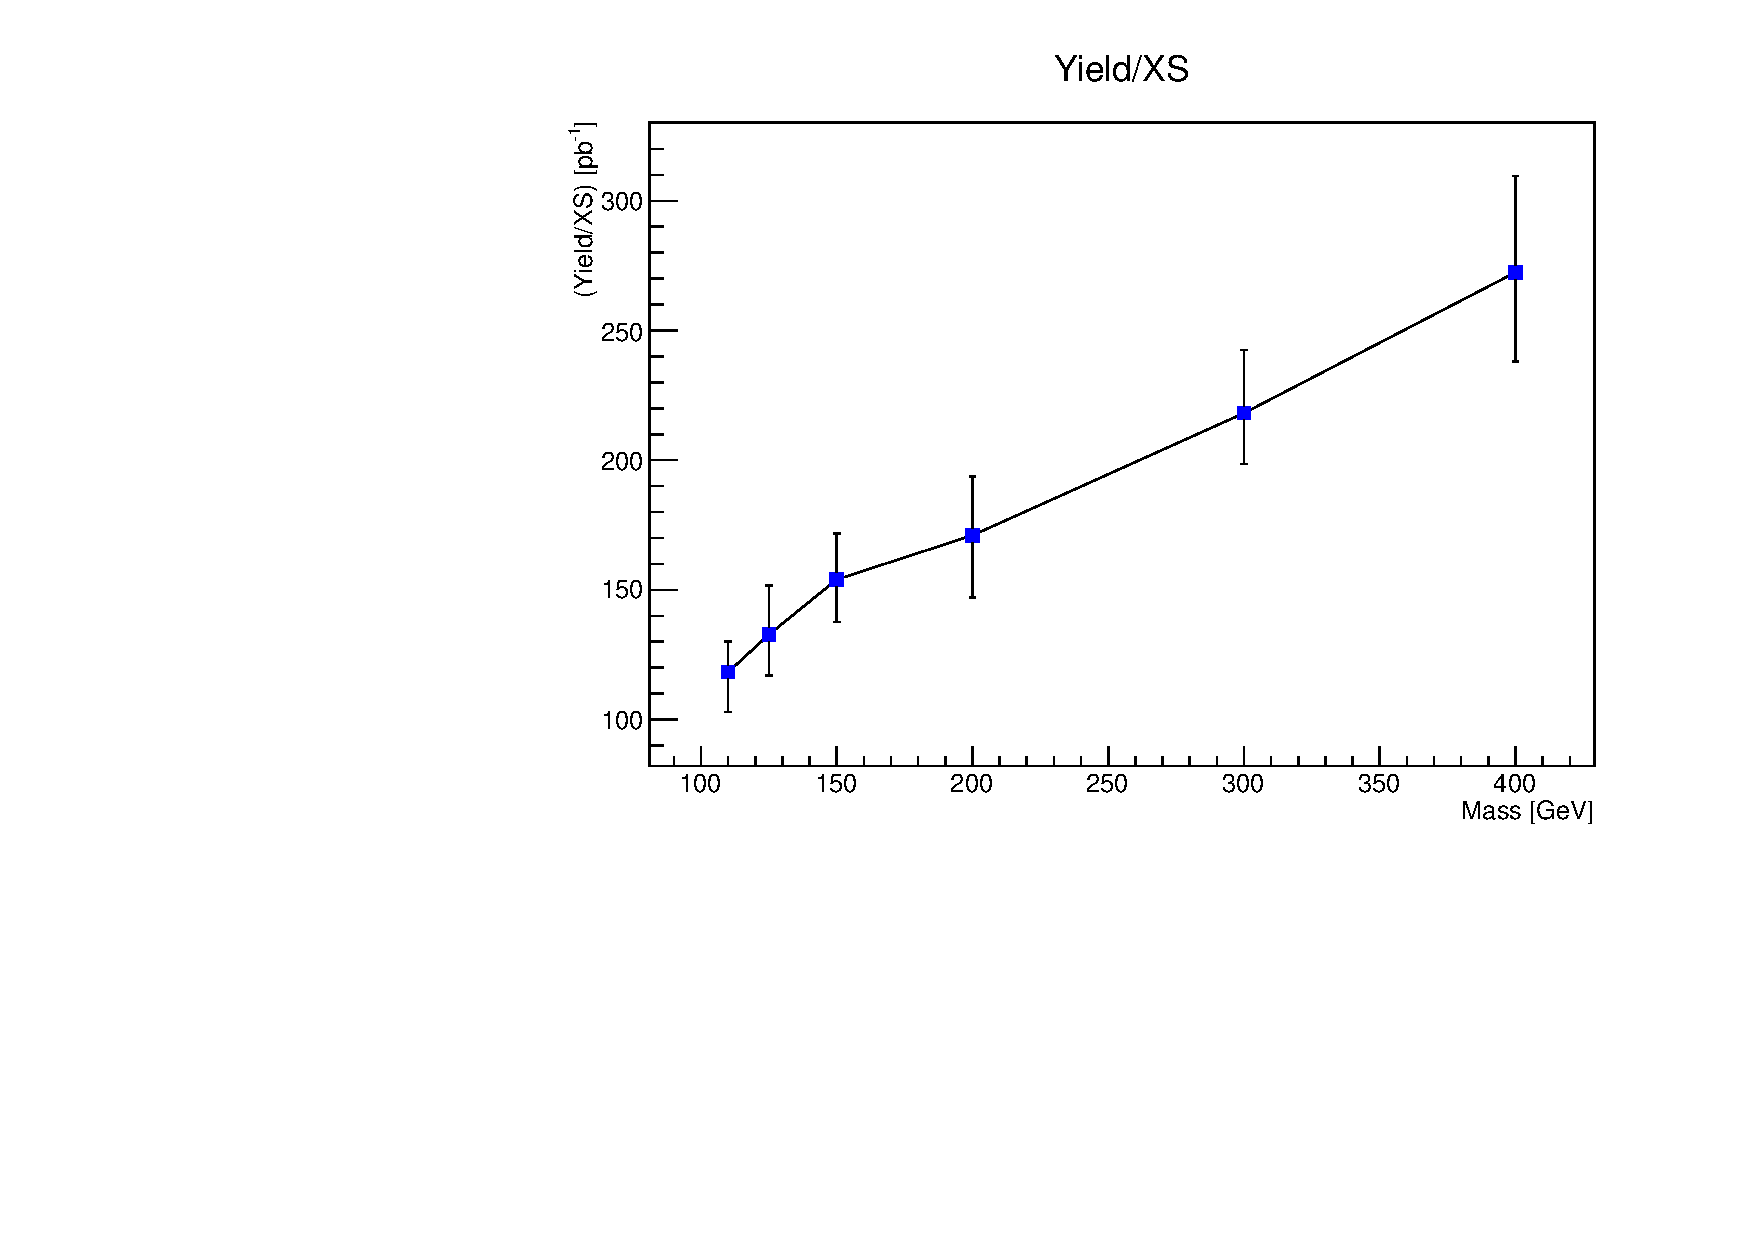
\includegraphics[clip=true,trim=0 0 0 30, width=1.2\textwidth]{TalkPics/invcomb021213/yieldoverxs.pdf}
  \end{columns}
\end{frame}

\begin{frame}
  \frametitle{Parked Data}
  \begin{block}{}
    \begin{itemize} 
    \item Jet $E_{T}>35(30) GeV$, $\Delta\eta_{jj}>3.5$, $m_{jj}>700 GeV$
    \item[-] Trigger with $E_{T}>30 GeV$ added for run D
    \item Good efficiency for visible and invisible VBF Higgs channels
    \item Plan to update result with parked data included after paper
    \end{itemize}
  \end{block}
\end{frame}

%TRIGGER AND DATASETS
\begin{frame}
  \frametitle{VBF Datasets and Trigger}
  \begin{columns}
    \column{.5\textwidth}
    \vspace{-0.2cm}
    \begin{block}{\scriptsize Datasets:}
      \scriptsize
      \begin{itemize}
      \item 8 TeV MET datasets
      \item[-] Total of 19.6 $fb^{-1}$
      \item MET filters are used to cut out events with mismeasured MET
      \end{itemize}
    \end{block}
    \vspace{-0.3cm}
    \begin{block}{\scriptsize Trigger:}
      \scriptsize
      \begin{itemize}  
      \item HLT\_DiPFJet40\_PFMET noMu65\_MJJ800VBF\_AllJets
      \item[-] VBF means $|\Delta \eta_{j_{1}j_{2}}| > 3.5 $
      \end{itemize}
    \end{block}
    \column{.5\textwidth}
    \centering
    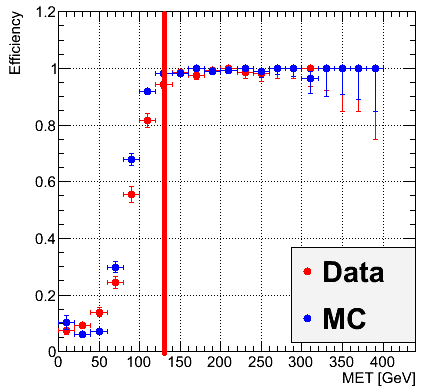
\includegraphics[height=.45\textheight]{TalkPics/METtrig.png}
    
    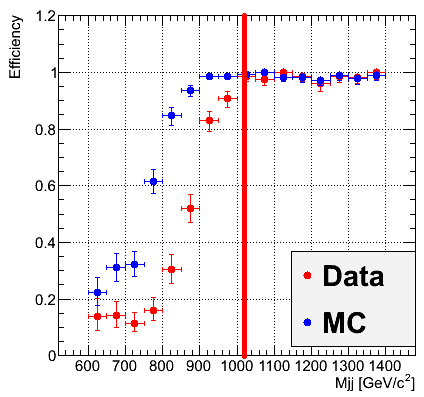
\includegraphics[height=.45\textheight]{TalkPics/Mjjtrig.png}
  \end{columns}
\end{frame}

%BACKGROUNDS
\begin{frame} 
  \frametitle{$W$+jets Background Estimation}
  \vspace{-0.4cm}
  \begin{columns}
    \column{.5\textwidth}
    \begin{block}{\scriptsize Background estimation formula:}
      \scriptsize
      \centering
      $N^{S}_{data} (W\rightarrow e/\mu) = (N^{C}_{data}-N^{C}_{bkg})\frac{N^{S}_{MC}}{N^{C}_{MC}}$  
    \end{block}
    \column{.5\textwidth}
    \begin{block}{\scriptsize $W \rightarrow \mu/ e$ Control Region Selection:}
      \scriptsize
      \begin{itemize}
      \item 1 tight muon/electron:
      \item MET $>130 GeV$
      \end{itemize}
    \end{block}
  \end{columns}
  \begin{columns}
    \column{.5\textwidth}
    \centering
    \scriptsize
    $W\rightarrow e\nu$
    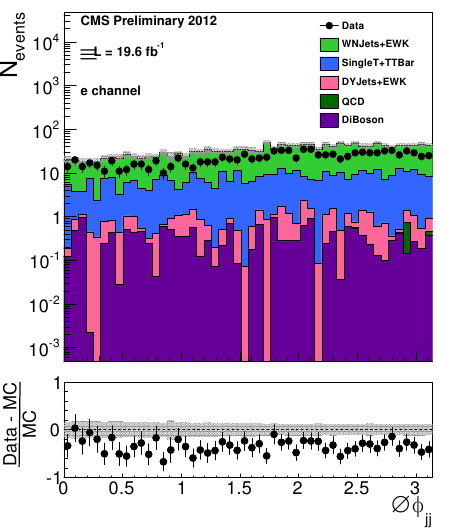
\includegraphics[width=\textwidth,height=.5\textheight]{TalkPics/iccms091013/dphijjwe.png}
    \column{.5\textwidth}
    \centering
    \scriptsize
    $W\rightarrow \mu\nu$
    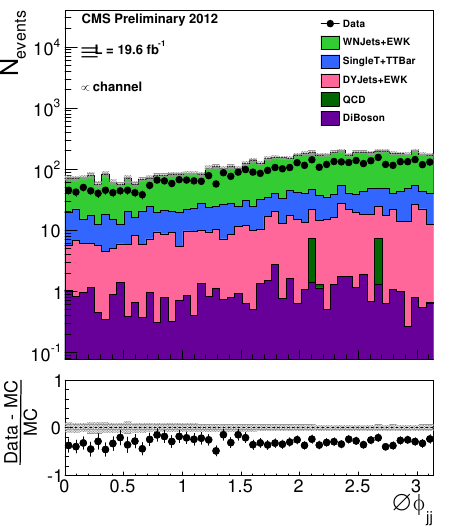
\includegraphics[width=\textwidth,height=.5\textheight]{TalkPics/iccms091013/dphijjwmu.png}
  \end{columns}
  \vspace{-0.2cm}
  
  \begin{columns}
    \column{.5\textwidth}
    \begin{block}{}
      \scriptsize
      \centering
      $N^{S}_{data} =$ $68.2\pm 9.2(stat.)\pm 13.1(syst.)$ events
    \end{block}
    \column{.5\textwidth}
    \begin{block}{}
      \scriptsize
      \centering
      $N^{S}_{data} =$ $67.2\pm 5.0(stat.) \pm 7.5 (syst.)$ events
    \end{block}
  \end{columns}
\end{frame}

\begin{frame}%!!PROBABLY DROP
  \frametitle{$W\rightarrow\tau_{\tiny had}\nu$ Background Estimation}
  \begin{columns}
    \column{.5\textwidth}
    \vspace{-0.3cm}
    \vspace{-0.2cm}
    \begin{block}{\scriptsize Background estimation formula:}
      \scriptsize
      \centering
      $N^{S}_{data} (W\rightarrow \tau\nu) = (N^{C}_{data}-N^{C}_{bkg})\frac{N^{S}_{W\rightarrow\tau\nu MC}}{N^{C}_{W\rightarrow\tau\nu MC}}$  
    \end{block}
    \begin{block}{\scriptsize $W\rightarrow \tau$ Control Region Selection:}
      \scriptsize
      \begin{itemize}
      \item Require signal region criteria except CJV
      \item Require 1 $\tau_{hadronic}$ candidate
      \item[-] No tau veto so this is a subsample of signal region without CJV
      \end{itemize}
    \end{block}
    \vspace{-0.2cm}
    \begin{block}{\scriptsize Result}
      \scriptsize
      \begin{itemize}
      \item $N^{data}_{W\rightarrow\tau\nu} = 54 \pm 16(stat.)\pm18(syst.)$
      \end{itemize}
    \end{block}
    \column{.5\textwidth}
    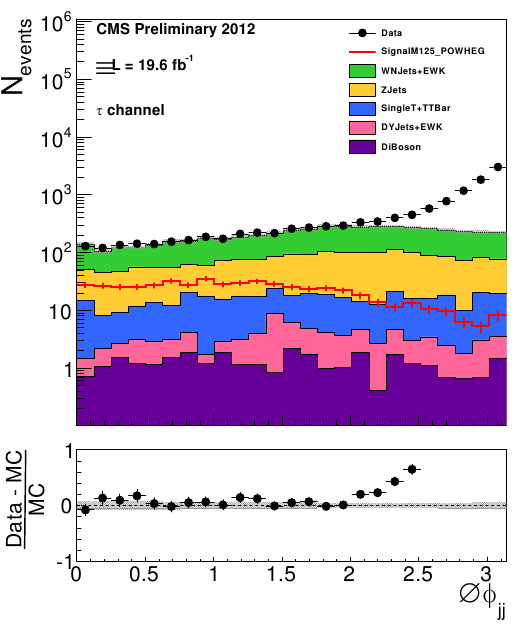
\includegraphics[width=\textwidth]{TalkPics/iccms091013/dphijjwtau.png}

  \end{columns}
\end{frame}


\begin{frame}%!!PROBABLY DROP
  \frametitle{$Z$+jets Background Estimation}
  \begin{block}{\scriptsize Z+jets background estimation formula:}
    \scriptsize 
    \centering
    $N^{S}_{data}(Z\rightarrow\nu\nu)=(N^{C}_{data} - N^{C}_{bkg})\frac{\sigma(Z\rightarrow\nu\nu)}{\sigma(Z/\gamma^{*}\rightarrow\mu\mu)}\frac{\epsilon^{S}_{VBF}/\epsilon^{C}_{VBF}}{\epsilon_{\mu\mu}}$
  \end{block}
  \begin{columns}
    \column{.5\textwidth}
    \begin{block}{\scriptsize $Z\rightarrow\nu\nu$ Control Region Selection:}
      \scriptsize
      \begin{itemize}
      \item Select $Z\rightarrow\mu\mu$ and extrapolate to $Z\rightarrow\nu\nu$
      \item[-] 2 tight muons with $60<M_{\mu\mu}<120$ GeV
      \item[-] MET after $Z$ candidate removed $> 130 GeV$
      \item[-] No additional veto muons/electrons
      \end{itemize}
    \end{block}
    \begin{block}{}
      \centering
      \scriptsize
      $N^{S}_{data}=102\pm30(stat.)\pm 14(syst.)$
    \end{block}
    \column{.05\textwidth}
    \column{.4\textwidth}
    \vspace{-.05cm}

    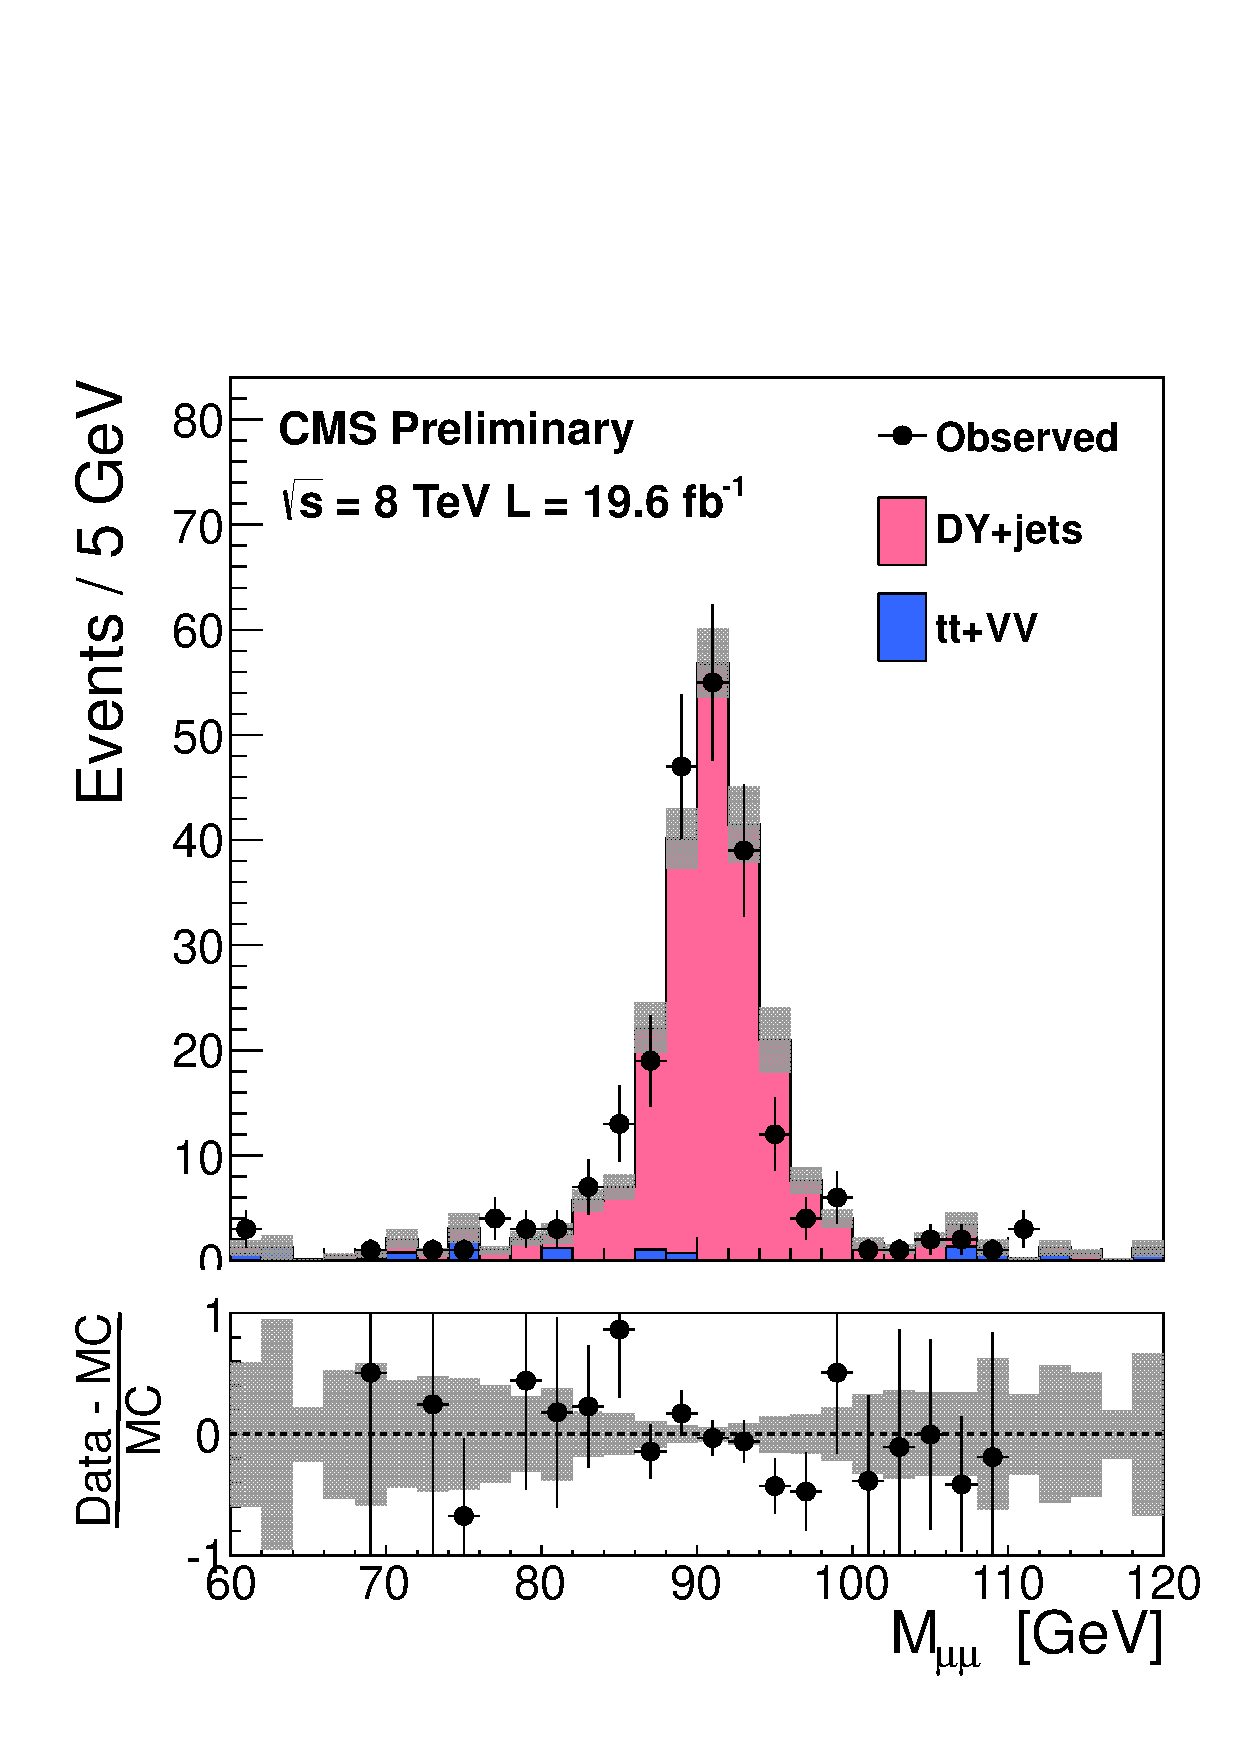
\includegraphics[width=.95\textwidth]{TalkPics/iccms091013/ZCtrlZMass.pdf}
  \end{columns}
\end{frame}

\begin{frame}%!!PROBABLY DROP
  \frametitle{Consistency Tests}
  \begin{columns}
    \column{.5\textwidth}
    \begin{block}{\scriptsize Method}
      \scriptsize
      \begin{itemize}
      \item To check $W/Z$+Jets estimates the $W\rightarrow\mu\nu$ sample is used to predict the other control region yields
      \item The predictions are consistent with the observed yields for all control regions
      \item[-] Some regions with significant QCD contamination show deviations
      \end{itemize}
    \end{block}
    \column{.5\textwidth}
    \centering
    \begin{block}{\scriptsize $W\rightarrow e\nu$ from $W\rightarrow\mu\nu$}
    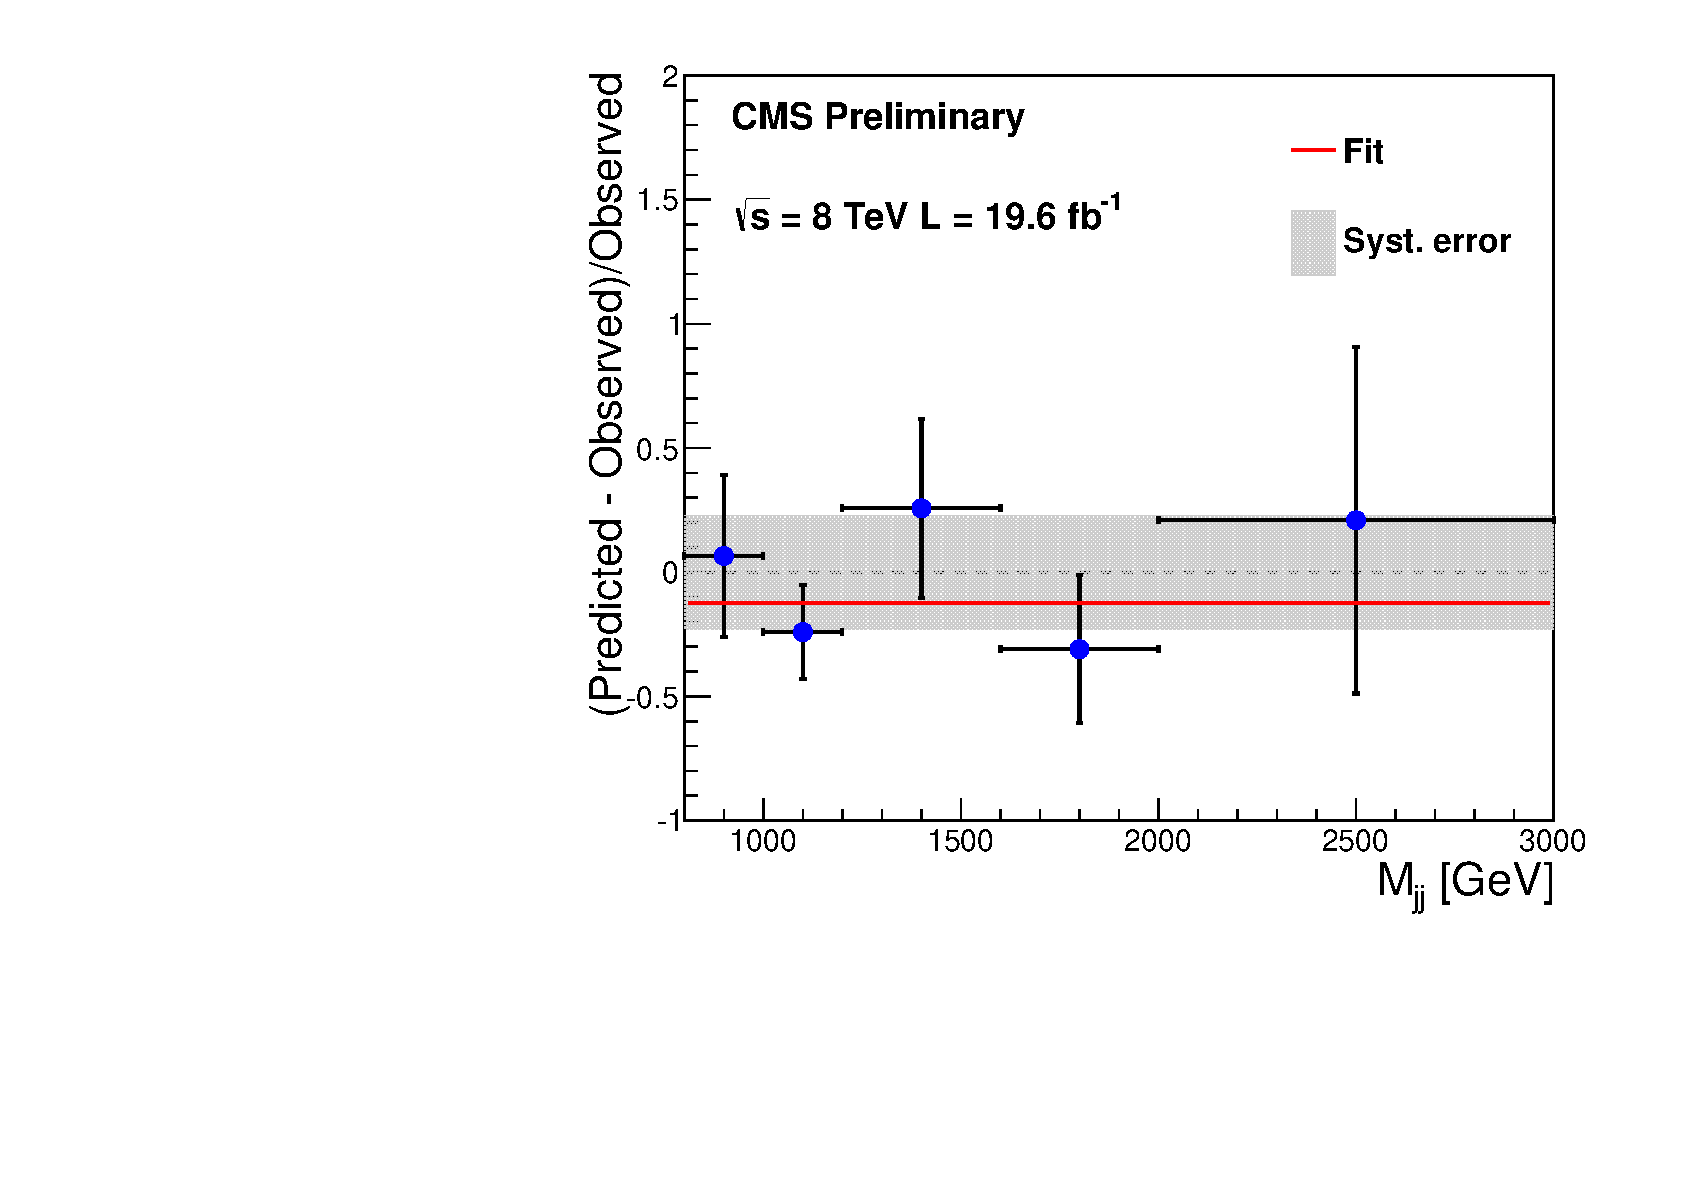
\includegraphics[width=\textwidth]{TalkPics/iccms091013/MJJ_Welnu_frac.pdf}
    \end{block}
  \end{columns}
\end{frame}

%OBJECTS
\begin{frame}
  \frametitle{Objects}
  \begin{columns}
    \column{.5\textwidth}
    \begin{block}{\scriptsize VBF Selections}
      \scriptsize
      \begin{itemize}
      \item \color{red} Applied to all regions
      \item 2 jets:
      \item[-] Both jets must pass loose PUJetID
      \item[-] $p_{T} > 50 GeV$,  $|\eta| < 4.7$
      \item[-] $|\Delta\eta|>4.2$ , $\eta_{j_{1}}*\eta_{j{_2}}<0$
      \item[-] $m_{jj} > 1100 GeV$
      \end{itemize}
    \end{block}
    \begin{block}{\scriptsize MET}
      \scriptsize
      \begin{itemize}
      \item Using Type 0 + 1 Corrections
      \end{itemize}
    \end{block}
    \column{.5\textwidth}
    \begin{block}{\scriptsize Electrons}
      \scriptsize
      \begin{itemize}
        \item Veto:
        \item[-] $p_{T}>10 GeV$, $|\eta<2.5|$
        \item[-] rel PF Iso $< 0.2$
        \item Tight:
        \item[-] $p_{T}>20 GeV$, $|\eta<2.5|$
      \end{itemize}
    \end{block}
    \begin{block}{\scriptsize Muons}
      \scriptsize
      \begin{itemize}
        \item Veto:
        \item[-] $p_{T}>10 GeV$, $|\eta<2.1|$
        \item[-] rel PF Iso $< 0.2$
        \item Tight: 
        \item[-] $p_{T}>20 GeV$, $|\eta<2.1|$
      \end{itemize}
    \end{block}
  \end{columns}
\end{frame}

\begin{frame}
  \frametitle{$W$+jets background $m_{T}$ plots}
  \begin{columns}
    \column{.33\textwidth}
    $e\nu$
    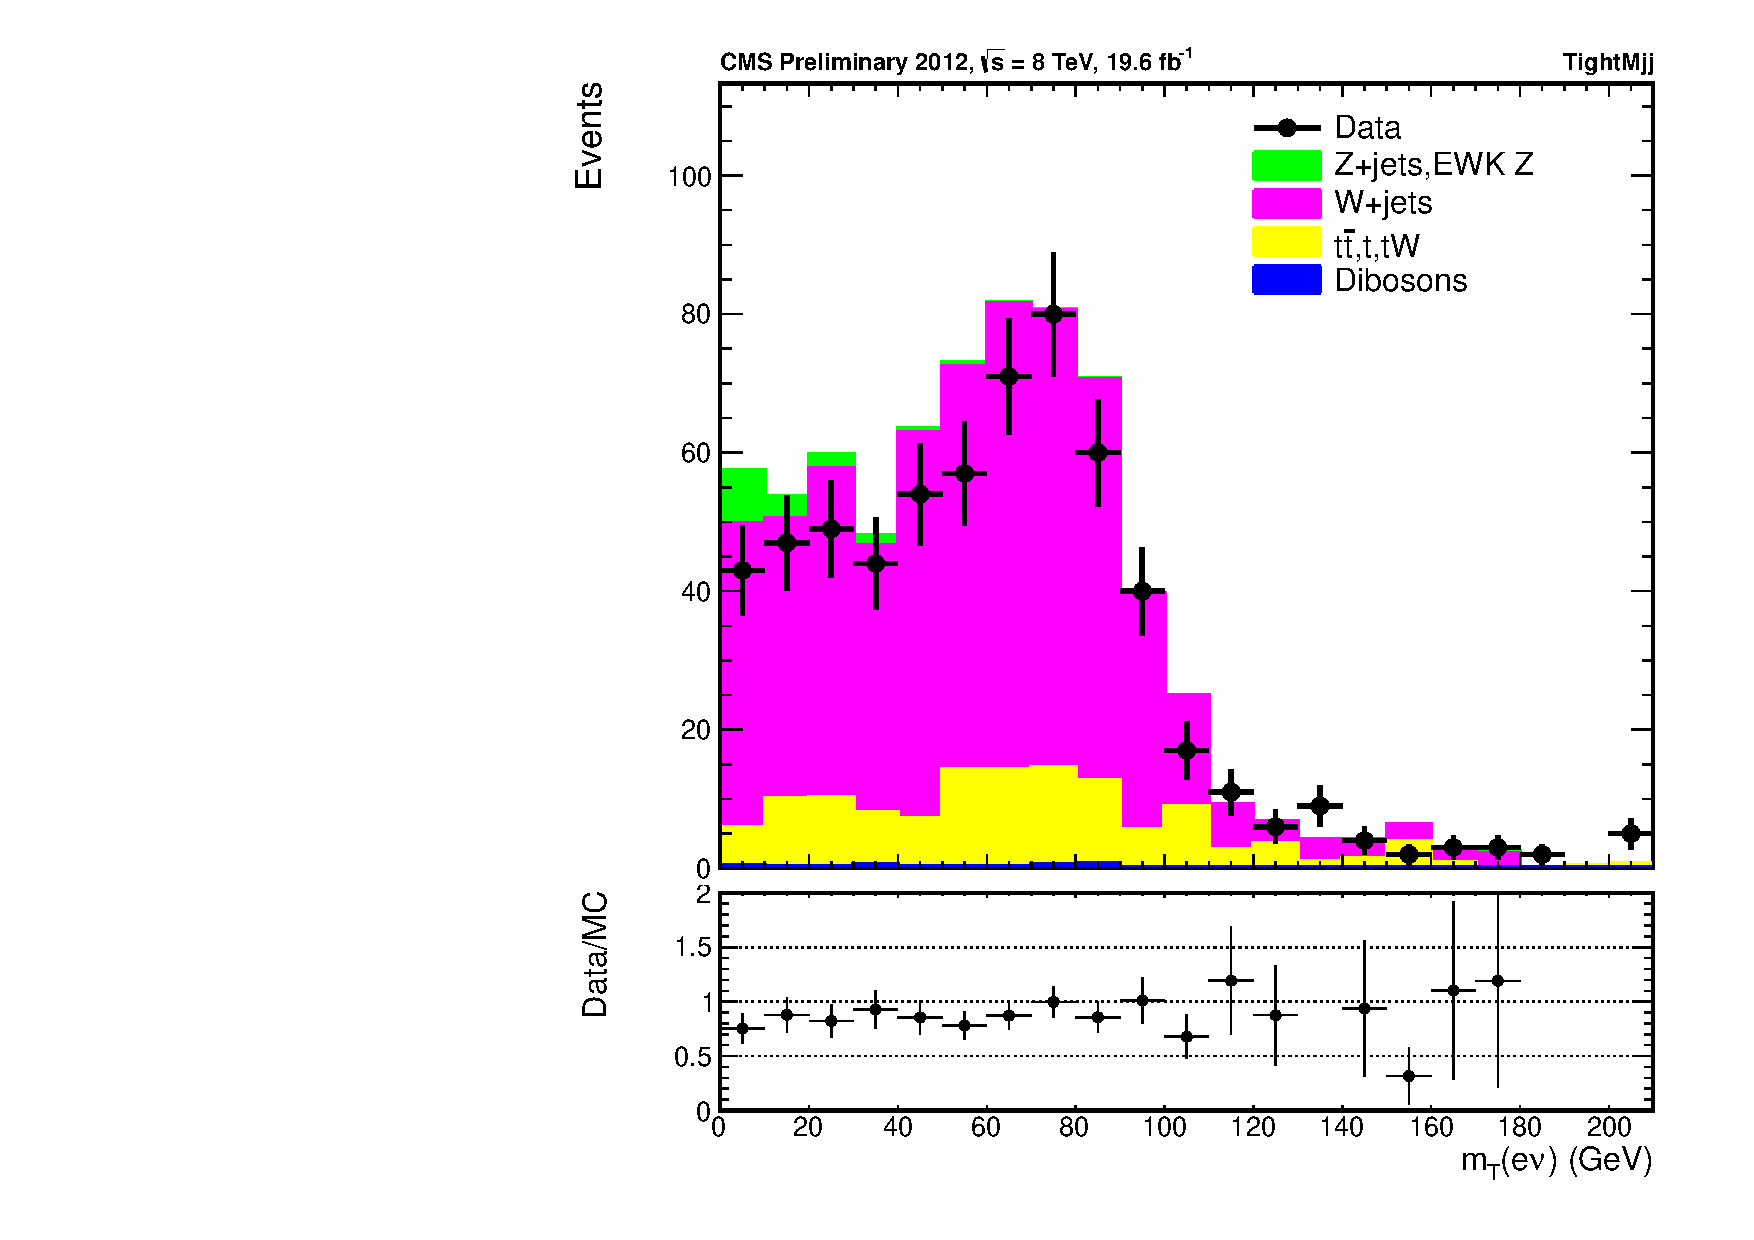
\includegraphics[width=\textwidth]{TalkPics/mt_enu_TightMjj.pdf}
    \column{.33\textwidth}
    $\mu\nu$
    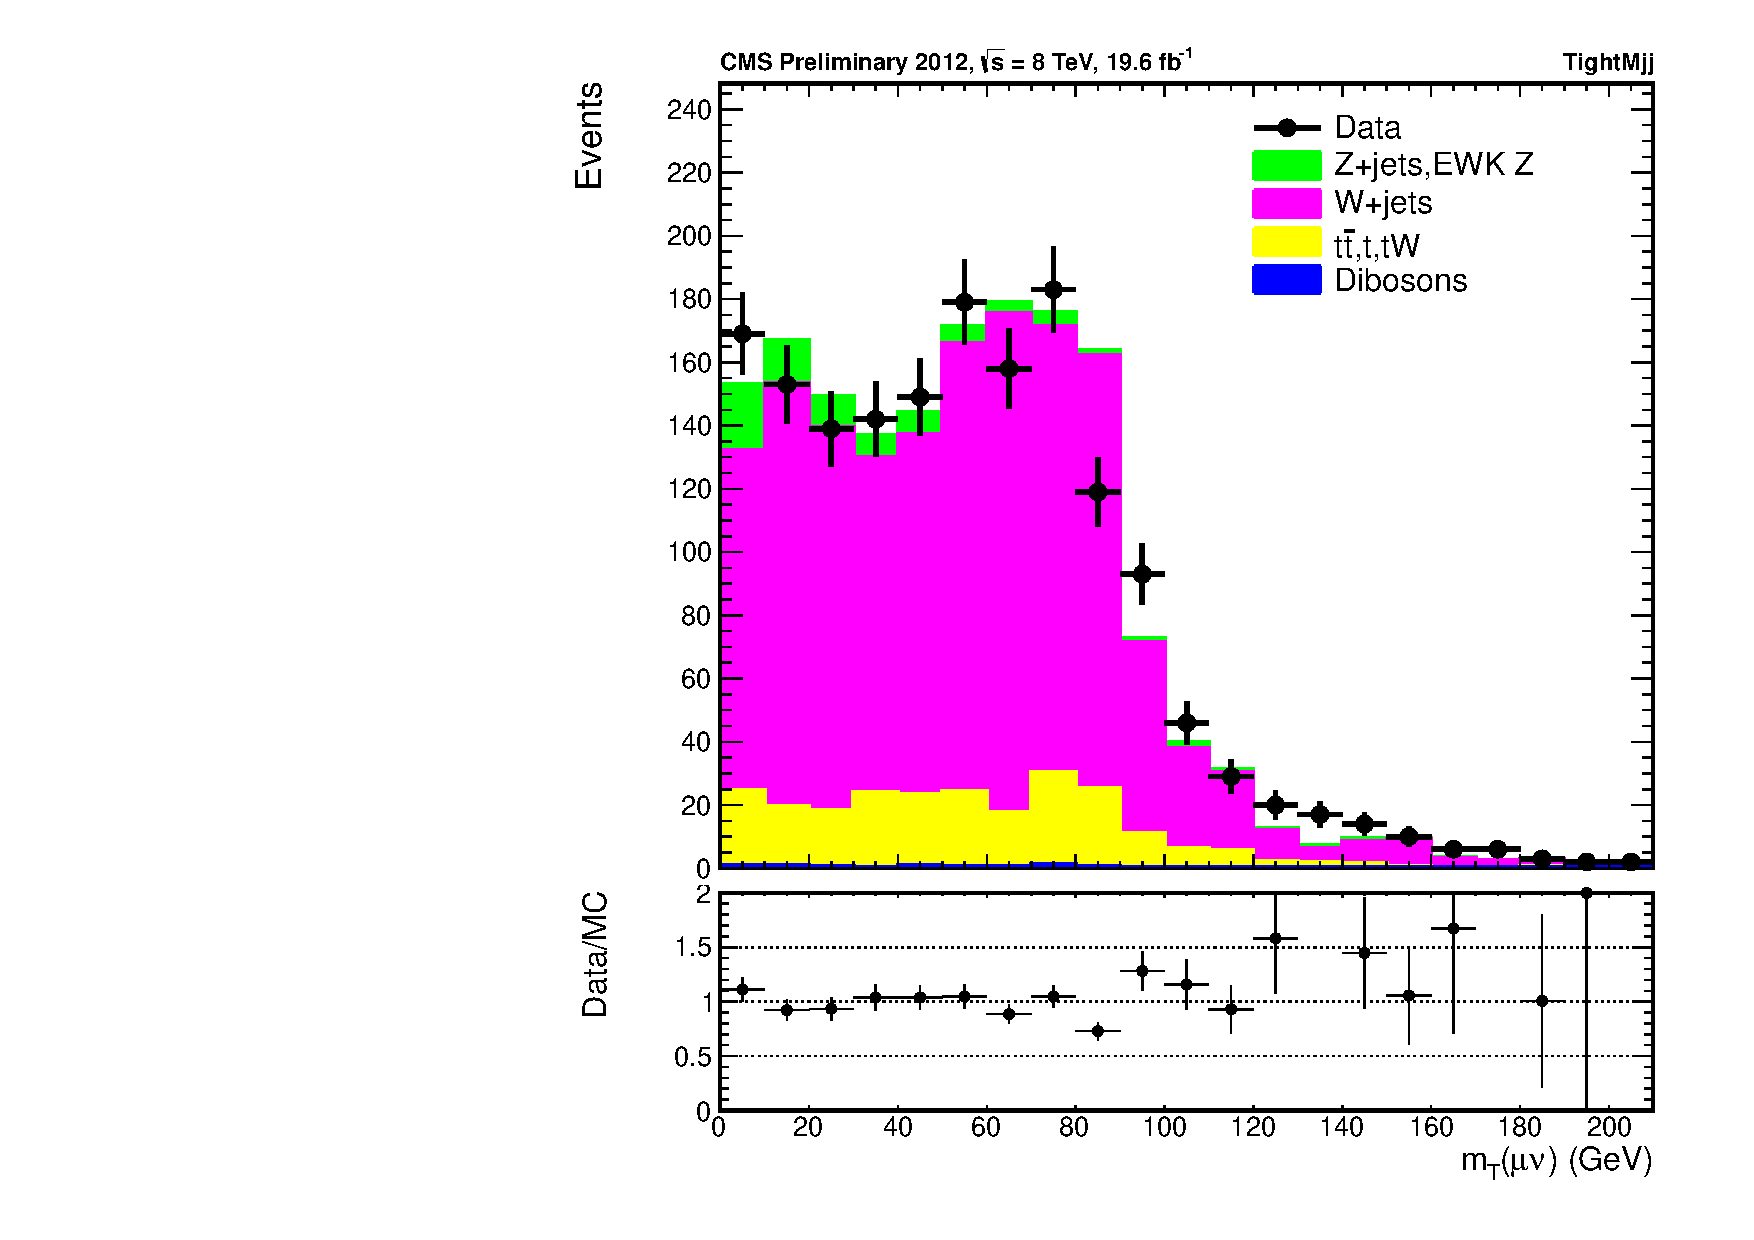
\includegraphics[width=\textwidth]{TalkPics/mt_munu_TightMjj.pdf}
    \column{.33\textwidth}
    $\tau\nu$
    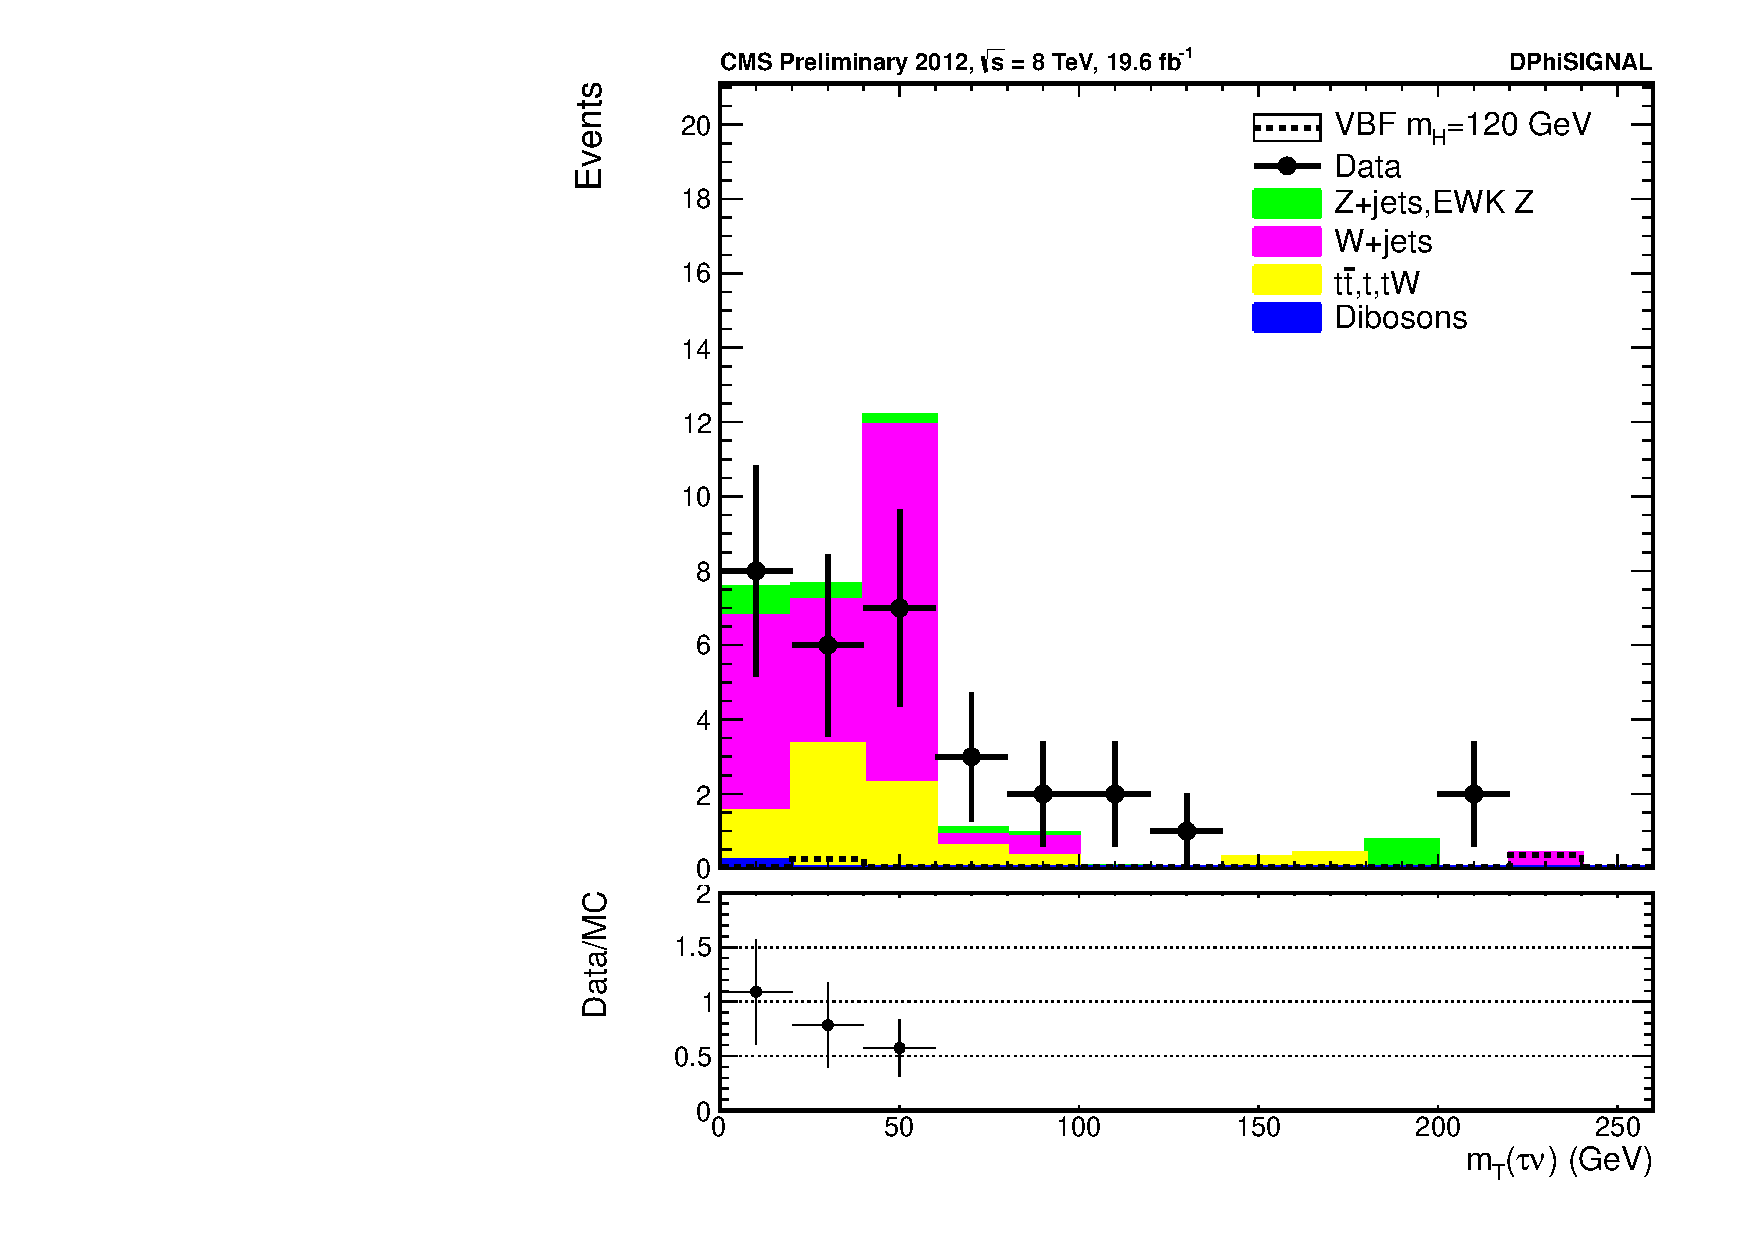
\includegraphics[width=\textwidth]{TalkPics/mt_taunu_2012_DPhiSIGNAL.pdf}
  \end{columns}
\end{frame}
\end{fmffile}
\end{document}
